%%%%%%%%%%%%%%%%%%%%%%%%%%%%%%%%%%%%%%%%%%%%%%%%%%%%%%%%%%%%%%%%%%%%%%%%
%                                                                      %
%     File: Thesis_Results.tex                                         %
%     Tex Master: Thesis.tex                                           %
%                                                                      %
%     Author: Andre C. Marta                                           %
%     Last modified :  2 Jul 2015                                      %
%                                                                      %
%%%%%%%%%%%%%%%%%%%%%%%%%%%%%%%%%%%%%%%%%%%%%%%%%%%%%%%%%%%%%%%%%%%%%%%%

\chapter{Results}
\label{chapter:results}

\section{Methodology}

In (D)\gls{tls} the key the authentication algorithm, the encryption algorithm, the
data integrity algorithm, as well as the associated key sizes for each are all defined in a \textit{ciphersuite}.
A ciphersuite defines the security properties of a \acrshort{tlsd} connection. For this reason, the terms
\textit{ciphersuite} and \textit{configuration} will be used interchangeably.

A \gls{tlsd} connection consists of two main phases:
\begin{enumerate}
  \item The peers authenticate one to another, agree on the data encryption and integrity
  algorithms that they will use and establish the shared keys. This part is known as the handshake protocol.
 \item The peers exchange the data securely, using the algorithms and keys negotiated in
the previous phase. This part is known as the record protocol.
\end{enumerate}

The relative cost of each phase depends on the chosen algorithms, as well as the amount of data
transferred. For this reason, it is important to evaluate the costs of both.

\acrshort{tlsd} has numerous possible configurations. Each one of those configurations is defined
in an \gls{rfc}. Each ciphersuite is assigned a unique identification number. \gls{iana} is responsible for
maintaining the full list of them. At the moment of this writing, there are over $300$ ciphersuites
defined for \gls{tlsd} \cite{IANA_ciphers_list:online}.

\textit{mbedTLS} implements a subset of those ciphersuites. As of version $2.7.0$, \textit{mbedTLS}
has a total of $161$ ciphersuites \cite{mbedTLS_ciphers_list:online}. Manual cost evaluation and
data analysis would greatly limit the scope of obtained results, as it would be very time consuming
and error-prone. For this reason, we developed tools that would automate the profiling and collection
of results.

In our work, we evaluated the \textit{mbedTLS's} implementation of the \gls{tls} protocol, thus obtained
metrics reflect the algorithm's implementations used within the library. 
We focused our analysis on two metrics: an estimated numbers of CPU cycles executed and time taken.
The obtained time metrics were not estimated, but rather values read directly from the processor's registers.
As we will show in later sections, the estimates reflect the real values.

There are well-established, industry-standard tools for collecting and analyzing the estimated computational costs,
such as the number of CPU cycles. Two of such tools are \textit{valgrind} and \textit{callgrind} and it's the ones that we used. 
Relying on such tooling allowed us to analyze the costs of \gls{tls} at both, the hiher and lower levels.
First, \textit{valgrind} allowed us to collect cost metrics for every part of \gls{tls}. Then, \textit{callgrind}
allowed us to visualize those costs and map the architecture of the codebase to relevant parts of \gls{tls} (\textit{i.e.}
which functions in the code correspond to which \gls{tls} operations).

Similarly, tools for reading performance related hardware counters directly from the processor exist. 
One of such tools is \gls{papi} \cite{dongarra2001using}.
After analyzing the estimated costs, we instructed the relevant parts of the code with \gls{papi}, in order to obtain
cost metrics directy from the processor's registers. More specifically, we measured time. A comparison of the estimates
and the real values showed that they are proportional one to another. 

\gls{tls}. First we collected a wide array of metrics with \textit{valgrind} and \textit{callgrind}, which allowed to
analyze the costs of \gls{tls} at both, high and low levels. After that, we studied the costs obtained by reading
the relevant counters directly from the processor and showed that they are proportional to the estimated ones.

In the next section we will analyze the evaluated metrics in detail, as well as describe their limitations.

\subsection{Evaluated Metrics and Limitations} \label{sec:eval-metrics-and-lims}

In this section we will describe the metrics that we evaluted, the environment in which the evaluation
was performed and the limitations of our approaches. We will present our descriptions in the same order
that we performed them: first estimating performance measurments with \textit{valgrind}, followed
by collecting values directly from the processor's counters with \textit{papi}.

\subsubsection{Estimation with Valgrind and Callgrind}

In order to estimate the number of executed cycles, we used \textit{valgrind}, more specifically
    its \textit{callgrind} tool. \textit{valgrind} runs the application on a synthetic CPU.
While running the code in that synthetic environment, it is able to insert instructions to perform
profiling and debugging.

In essence, \textit{valgrind} is a virtual machine, using \gls{jit}
compilation techniques, such as dynamic recompilation. Dynamic recompilation is a
feature where some part of the program is recompiled during execution.

The \textit{valgrind} tool consists of two parts, the \textit{valgrind core} and the \textit{tool
plugin}. The \textit{valgrind core} transforms the machine code into a simpler form called
\gls{ir}. The \gls{ir} code is then passed to the \textit{tool plugin}, which modifies the
\gls{ir} code as needed, typically by instrumenting it. This modified \gls{ir} code is then passed back to the
\textit{valgrind core}, which transforms it back into machine code. That recompiled machine code  will then run on the
host CPU (the \gls{jit} compilation step). This process is illustrated in Figure \ref{fig:how_valgrind_works}.

\begin{figure}
  \centering
  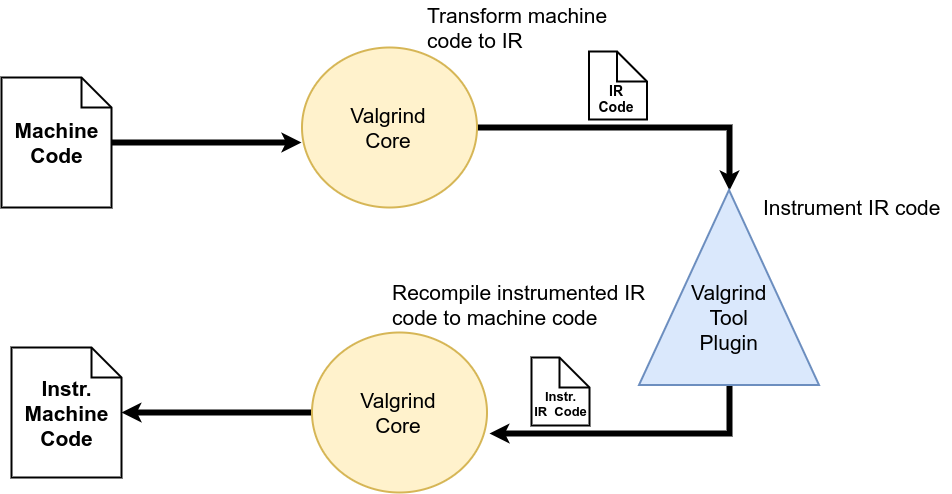
\includegraphics[width=1.0\textwidth]{img/how_valgrind_works.png}
  \centering \caption{\label{fig:how_valgrind_works} How Valgrind works}
\end{figure}

In our case, the \textit{tool plugin} is \textit{callgrind}. Among other metrics, \textit{callgrind}
collects the number of executed instructions, L1/L2 caches misses (the caches are simulated), and branch
prediction misses. The metrics collected by \textit{callgrind} can then be loaded into \textit{kcachegrind}
to visualize and analyze the performance results. One of such results is the estimate of the number of executed CPU cycles.
\textit{callgrind} and \textit{kcachegrind} are widely in conjunction for performance analysis and optimization
of programs. In order to count the number of executed CPU cycles, we derived a formula from
the one that is used by \textit{kcachegrind}.

The number of executed cycles
presented by \textit{kcachegrind} is an estimate, which might not correspond to the real value.
Although undocumented, we found the formula that estimates the number of executed CPU cycles in
\textit{kcachegrind}'s source code \cite{cachegrind_source:online}.
It uses the
following formula: $CEst = Ir + 10*Bm + 10*L1m + 20*Ge + 100*L2m + 100*LLm$, where

\begin{itemize}
  \item $CEst$ - estimated CPU cycles
  \item $Ir$ - instruction fetches
  \item $Bm$ -  mis-predicted branches (direct and indirect)
  \item $Ge$ - number of global bus events
  \item $L1m$ - total L1 cache misses (instruction fetch, data read and data write)
  \item $L2m$ - total L2 cache misses (instruction fetch, data read and data write)
  \item $LLm$ - total last-level cache misses (instruction fetch, data read and data write)
\end{itemize}

\textit{Callgrind} only simulates L1 and L2 caches, making $LLm=0$, therefore the actual formula
used by \textit{KCachegrind} (when used with \textit{Callgrind} output) is:
$CEst = Ir + 10*Bm + 10*L1m + 20*Ge + 100*L2m$.

$Ge$ is a useful metric when synchronization primitives are present, since it counts the number of
atomic instructions executed. For example, on the x86 and x86\_64 architectures, these are
instructions using the \textit{lock} prefix. In our evaluation, only single-threaded code was used, therefore
reason we did not measure $Ge$. This further simplified the formula used by \textit{kcachegrind} to
$CEst = Ir + 10*Bm + 10*L1m + 100*L2m$.

In order to estimate the number of CPU cycles, we developed tooling that parsed the metrics output by
\textit{callgrind} and input them into the \textit{kcachegrind}'s formula. All of the evaluations were performed in
our local machine, with its relevant characteristics shown in table \ref{table:local-machine}.

\begin{table}[]
\begin{tabular}{|l|l|}
\hline
Processor            & Intel(R) Core(TM) i7-4700HQ CPU @ 2.40GHz \\ \hline
L1 Instruction Cache & 32768 B, 64 B, 8-way associative          \\ \hline
L1 Data Cache        & 32768 B, 64 B, 8-way associative          \\ \hline
LL Cache             & 6291456 B, 64 B, 12-way associative       \\ \hline
\end{tabular}
\centering \caption{\label{table:local-machine} Local machine's characteristics}
\end{table}

\subsubsection{Reading Values From Processor Counters with PAPI}

In order to obtain the actual processor time spent on various parts of \gls{tls} 
we used \gls{papi}. Hardware designers added registers to the processors to measure various 
aspects of its function. Those registers act as performance counters that count specific
signals related to processor's funtion, such as the number of instructions executed and total
time elapsed. \gls{papi} provides a standard interface for accessing those counters.

\gls{papi} provides interfaces to measure both, virtual and processor time. \textit{Real time},
also known as \textit{wall clock time} is total elapsed time, including the time slices used
by ohter processes, as well as the time spent while the process was blocked, while, for example,
waiting for I/O operations to complete. \textit{Virtual time}, also known as \textit{user time},
is amount of time spent in user mode within the process (\textit{i.e.} time spent in kernel mode is not included). 
This measure is the actual CPU time used in executing the process and does not include time slices 
used by other processes or the time the process spends blocked. For our purposes, only the \textit{virtual time}
was relevant and it was the one that we measured.

Just like with \textit{valgrind}, all of our \gls{papi} evaluations were perfomed on the machine
described in table \ref{table:local-machine}. However, in order to keep the metrics consistent,
we disabled Intel Turbo Boost \cite{charles2009evaluation} and fixed the processor's speed to the lowest available frequency
of $800Mhz$.

\subsubsection{Limitations}

The metrics obtained with \textit{valgrind}/\textit{callgrind} are just estimated values, which do not
necessarily reflect the real ones. For this reason, we complemented them with \gls{papi} measures, which
are read directly from the processor's registers.

We did not collect any measures on typical \gls{iot} processors. Despite that, the presented metrics are are still
relevant. If collected on an \gls{iot} processor, the metrics would maintain a similar proportion, thus
the conclusions and analysis presented would still hold true. Moreover, it is possible to run \textit{callgrind}
on an \gls{iot} processor (either manually or using our automated tooling) and use those metrics for more accurate 
and device-specific CPU cycle estimation. The same is true for \gls{papi}. In the next section we will describe which we tools developed in order 
to collect the metrics presented in this work. It is possible to use those tools in a local environment to 
automate metric collection.

\subsection{Developed Tools}

\textit{mbedTLS 2.7.0} provides numerous possible configurations for a \gls{tls} connection. It would be unfeasible to
perform a thorough and precise evaluation of its \gls{tls} implementation manually. For this reason, we developed a set
of tools to automate those tasks. In general, the developed tools served one of two purposes: metric collection and
collected metric analysis, for both \textit{valgrind} and \gls{papi}. All of the developed tooling is open-source
and available online.

In order to collect the relevant metrics, we developed automated tools that would run a client-server connection with a specified set
of ciphersuites and save the collected metrics for later analysis. \textit{callgrind} outputs files with the profiling information,
so we used those files directly \cite{iluxonch23:online}. As for the \gls{papi} results, we programmed a custom metrics collector that 
would group the metrics and save them in \textit{JSON} format \cite{iluxonch67:online}. In order to isolate ciphersuites with unique encryption
algirithms for the purposes of encryption algorithms cost analsys, we developed a command-line tool
that performs that filtering \cite{iluxonch73:online}.

After being collected, the metrics were ready to be analyzed. For \textit{callgrind} we developed tools that would use the collected 
measurments to estimate the number of CPU cycles for the specified \textit{mbedTLS} functions \cite{iluxonch23:online} \cite{iluxonch44:online}. 
\textit{mbedTLS} functions either implement \gls{tls} security services
(\textit{e.g.} authentication) or primitives used by \gls{tls} them (\textit{e.g.} \gls{rsa} signature creation).
After associating the function name(s) to each relevant security service and primitive, their costs could be studied. 
Our tools allow to analyze the collected metrics both, individually (\textit{e.g.} compute the cost the handshake for a specific ciphersuite), and in conjunction (\textit{e.g.}
compute the average cost of the handshake for all of the ciphersuites that use a specific key exchange method).
A separate set of tooling with equivalent functionality was developed in order to analyze the time results obtained with \gls{papi} \cite{iluxonch67:online}.

In order to collect the \textit{valgrind} metrics, no modification of \textit{mbedTLS}'s source code was necessary. To obtain the time measurments, the relevant
parts of the \textit{mbedTLS} code had to be instrumented with \gls{papi} \cite{iluxonch24:online}. In both cases, dedicated client and server
executables were developed \cite{iluxonch24:online}. Each executable accepts two arguments: the \textit{id} of the ciphersuite to use and the number of bytes to transmit to the other
peer. This set up allowed us to profile the costs of all security services for each one of the ciphersuites.
   \cite{iluxonch24:online}

\section{Results and Data Analysis}

The \gls{tlsd} protocol consists of two sub-protocols: the Handshake protocol and the Record protocol.
During the Handshake protocol, the peers authenticate one to another, agree on the data encryption and integrity
algorithms and establish the shared keys. During the Record protocol the peers exchange the data securely,
using the algorithms and keys negotiated during the Handshake protocol. Those algorithms support the security
services provided by \gls{tlsd}. For example, peer entity authentication is usually offered by algorithms, such
as \gls{rsa} or \gls{ecdsa}. The cost of the Handshake phase depends on the security services used. The cost
of the Record phase depends on the amount of data transmitted.

The core of the Record protocol is the use of a symmetric encryption algorithm (\textit{e.g} AES), used to
provide confidentiality and an \gls{hmac} algorithm, used to provide data integrity and data origin authentication.
The \gls{hmac} algorithm is not used if the symmetric encryption algorithm is an \gls{aead} cipher, which already
provides data integrity guarantees. Each encryption algorithm has a few possible varieties (\textit{e.g.} the CBC, GCM and CCM modes in AES)
and key sizes  (\textit{e.g.}, $128$ and $256$ bit for AES). The same is true for \gls{hmac} algorithms, which
have a well defined \gls{mac} function, key size and output length. The performance of symmetric encryption
algorithms and hash functions has been studied in detail by existing work \cite{nadeem2005performance} \cite{mathew2010performance}.
There is an approximately linear relation between the amount of data encrypted and the the cost, as we 
show in Section \ref{sec:confid-costs}.

The previous paragraph does not apply to the Handshake protocol. In this part, there is more variety in the
computational cost outcomes. There are a few reasons for that:

\begin{itemize}

  \item Asymmetric cryptography algorithms are used to provide security services of authentication
  and \gls{pfs}. For each algorithm, there are significantly more possible key sizes, when compared to
  symmetric encryption algorithms. Theoretically there is an infinite number of them, however practical limits exist\cite{lenstra2004key}.

  \item In \gls{tlsd}, various algorithms, in various combinations can be used to provide authentication and \gls{pfs}.
  Two types of public key algorithms than can be used: \gls{ecc}-based and non-\gls{ecc}-based. It is also possible
  to have authentication without asymmetric cryptography. \gls{psk}-based ciphersuites allow peers to
  authenticate one to another by the means of a shared secret. This shared secret is then input to the \gls{prf}
  in the premaster key generation, without the use of public key cryptography.

  \item The use of asymmetric cryptography leads to asymmetric costs (\textit{i.e.} distinct costs) for the client and the server. The costs of asymmetric
  encryption algorithms vary greatly depending if the public or the private key is used. Also, while \gls{ecc}
  algorithms tend to have a smaller computational footprint, this is not always the case.
  Some operations (\textit{e.g} signature verification) is faster on the non-\gls{ecc} counterparts.
  It is important to consider those factors, when for example, only one of the peers is constrained, since the costs for the client and the server will be different.
  In the Record phase we do not have that problem, since the costs of \gls{hmac} and encryption/decryption in
  symmetrical encryption algorithms is approximately the same.

\end{itemize}

Another cryptographic operation that is done in the Handshake phase is \gls{prf} keying material generation. This part, however,
does not have a major influence on the computational costs and is the same for both peers, since it is essentially
hashing operations.

It is clear that the Handshake protocol is significantly more complex, with more possible cost variations.
Furthermore, existing work neither evaluated the costs of individual security services of \gls{tls}, nor
their various combinations. For this reason, our work is concentrated around the Handshake protocol.

This section as structured as follows. Section \ref{sec:sls} describes the various security levels used for evaluation. 
Section \ref{sec:ss-overview}
presents an overview of the costs of authentication and \gls{pfs}. Section \ref{sec:psk-cost-analysis} discusses the costs of symmetric (or \gls{psk})
authentication. In Section \ref{sec:asym-algs-analysis} we analyze the costs of asymmetric authentication. We begin by analyzing the cost of \gls{rsa}'s
and \gls{ecdsa}'s  operations and then put everything together and present the authentication cost for each key exchange method (thus, for each ciphersuite).
Section \ref{sec:pfs-costs} does a similar analysis, but his time for the cost of \gls{pfs}. Here, once again, we begin by analyzing the costs of
\gls{ecdh} and \gls{dh}, after which we use that information to arrive at the \gls{pfs} cost for each key exchange method (thus, for each ciphersuite).
Section \ref{sec:tls-hs-cost} puts the information from the previous sections together and analyzes the cost of the \gls{tls} handshake as a whole.
We do both, present actual handshake cost values obtained by profiling its cost directly, and show how to use the information from the previous sections to 
arrive to those cost values without the need of executing and profiling the handshake costs directly. We decompose \gls{tls} costs into a single formula.
In Section \ref{sec:confid-costs} we discuss costs of confidentiality in \gls{tls} and compare the performance of all of the symmetric encryption algorithms
present in \textit{mbedTLS 2.7.0}. Having analyzed the estimates obtained with \textit{valgrind}, we will turn our focus to time costs obtained with \gls{papi}.
Section \ref{sec:papi-handshake} presents handshake time measurments collected with \gls{papi} and compares them to
the \textit{valgrind} ones from Section \ref{sec:tls-hs-cost}. As we will show, they are similar. In Section \ref{sec:papi-valgrind-ratios} we go further,
and compare \gls{papi}'s ratios of related algorithm opearations to the \textit{valgrind} ones. In essence, we will compare \gls{papi}'s results to the valgrind
one's analyzed in Sections \ref{sec:asym-algs-analysis} and \ref{sec:pfs-costs}, and once again show that they are similar.
Finally, in section \ref{sec:ss-cost-conclusions} we present some conclusions.

\subsection{Security Levels} \label{sec:sls}

We performed evaluation under various security levels, which are presented in table \ref{table:tls-sec-lvls}.
The defined security levels are based on modern day security practices. The equivalence between symmetric and asymmetric
key sizes  is based on table \ref{table:ecc-key-sizes}. It shows approximate comparable key sizes for symmetric
and asymmetric key algorithms based on the best known algorithms for attacking them\cite{RFC4492}.

Unfortunately, mbedTLS does not have
the exact ECC curves for the  key sizes with the values specified in the the table. For this reason, for \gls{ecc}
we choose the closest larger value available.


\begin{table}[]
\begin{tabular}{|l|l|l|l|}
\hline
Security Level & Symmetric & ECC & DH/DSA/RSA \\ \hline
\textit{S1}    & 80        & 163 & 1024       \\ \hline
\textit{S2}    & 112       & 233 & 2048       \\ \hline
\textit{S3}    & 128       & 283 & 3072       \\ \hline
\textit{S4}    & 192       & 409 & 7680       \\ \hline
\textit{S5}    & 256       & 571 & 15360      \\ \hline
\end{tabular}
\centering \caption{\label{table:ecc-key-sizes} Comparable symmetric and asymmetric key sizes (in bits)}
\end{table}

\begin{table}[]
  \begin{tabular}{|l|l|l|l|l|}
  \hline
                                                                       & \textbf{low} & \textbf{normal} & \textbf{high} & \textbf{very high} \\ \hline
  \begin{tabular}[c]{@{}l@{}}Symmetric Key Size\\ (bits)\end{tabular}  & 128               & 128               & 192\addtocounter{footnote}{1}\addtocounter{footnotesintable}{1}\footnotemark[\thefootnote]             & 256            \\ \hline
  \begin{tabular}[c]{@{}l@{}}RSA/DH/DSA Key Size\\ (bits)\end{tabular} & 1024              & 2048              & 4092          & 8192           \\ \hline
  \begin{tabular}[c]{@{}l@{}}ECC Key Size\\ (bits)\end{tabular}        & 163 \addtocounter{footnote}{1}\addtocounter{footnotesintable}{1} \footnotemark[\thefootnote]               & 233 \addtocounter{footnote}{1}\addtocounter{footnotesintable}{1}\footnotemark[\thefootnote]               & 317\addtocounter{footnote}{1}\addtocounter{footnotesintable}{1}\footnotemark[\thefootnote]             & 420\addtocounter{footnote}{1}\addtocounter{footnotesintable}{1}\footnotemark[\thefootnote]              \\ \hline
  HMAC                                                                 & SHA-256           & SHA-256           & SHA-384       & SHA-512  \addtocounter{footnote}{1}\addtocounter{footnotesintable}{1}\footnotemark[\thefootnote]      \\ \hline
  \end{tabular}
  \centering \caption{\label{table:tls-sec-lvls} Security levels used in evaluation}
  \end{table}

\addtocounter{footnote}{-\thefootnotesintable}
\addtocounter{footnote}{1}\footnotetext[\thefootnote]{The closest value available in mbedTLS 2.7.0 (rounded up) is $256$ bit}
\addtocounter{footnote}{1}\footnotetext[\thefootnote]{The closest value available in mbedTLS 2.7.0 (rounded up) is $224$ bit}
\addtocounter{footnote}{1}\footnotetext[\thefootnote]{The closest value available in mbedTLS 2.7.0 (rounded up)is $256$ bit}
\addtocounter{footnote}{1}\footnotetext[\thefootnote]{The closest value available in mbedTLS 2.7.0 (rounded up) is $384$ bit}
\addtocounter{footnote}{1}\footnotetext[\thefootnote]{The closest value available in mbedTLS 2.7.0 (rounded up) is $512$ bit}
\addtocounter{footnote}{1}\footnotetext[\thefootnote]{The strongest hash function available in mbedTLS is SHA-384}

We based the \textbf{normal} security level on the current most used \gls{tls} configuration on the internet \cite{QualysSS90:online}.
We could not find any typical values used in the sphere of \gls{iot}. In all of the security levels, a
certificate chain with two certificates is used: the \gls{ca}'s certificate
and the server's certificate. Only server-side authentication is used, since this is the most common scenario.
We decided to use the smallest possible certificate chain, consisting of two certificates. This is not the norm
on the internet, where the chain size is larger. However, adding more certificates to the chain would not provide additional
information, since the extra cost of additional certificates in the chain can be computed by adding the costs of
making/verifying additional signatures and parsing the certificates.

For all security levels, the server certificates are either
signed with a $2048$ bit \gls{rsa} with SHA-256 secure signing scheme \cite{RFC8017}, or with a $256$ bit \gls{ecdsa} with SHA-256 secure
signing scheme (\textit{secp256r1} curve) \cite{RFC6979},
depending on the ciphersuite.
The chosen signature algorithm and key size is based on the usual \gls{ca} practices. For example,
Google's root certificates with common names \textit{Google Internet Authority G2} and \textit{Google Internet Authority G3}
use this set up\cite{GoogleIn11:online}.

The server's certificates, however, contained public keys of different sizes, according to the certificate type.
For this reason, it is possible to deduce the cost of the \gls{ca}'s signature using a different algorithm with a
different key. For the \textbf{normal} security configuration, the certificates used by the server are as follows:

\begin{itemize}
  \item if \gls{rsa} authentication is used, the server's certificate will contain an $2048$ bit \gls{rsa} key;
  \item if \gls{ecdsa} authentication is used, the server's certificate will contain a $256$ bit \gls{ecc} key (\textit{secp256r1} curve);
  \item if \gls{dh} is used for \gls{pfs}, the negotiated key will be $2048$ bit long;
  \item if \gls{ecdh} is used fro \gls{pfs}, the negotiated key will be $256$ bit long and the \textit{secp256r1}
  curve will be used. The choice of this curve was based on the preferred curve order of Google Chrome $67$, the most
  used web browser in the world\cite{BrowserS4:online}.
\end{itemize}

Table \ref{table:sls-config-info} contains a the certificate configuration and key size information for all of the
security levels. The key sizes are presented in bits.

\begin{table}[]
\begin{tabular}{|l|l|l|l|l|}
\hline
               & \textbf{low} & \textbf{normal} & \textbf{high} & \textbf{very high} \\ \hline
RSA Key Size   & 1024         & 2048            & 4092          & 8192               \\ \hline
ECDSA Key Size & 192          & 256             & 384           & 521                \\ \hline
DH Key Size    & 1024         & 2048            & 4092          & 8192               \\ \hline
ECDH Key Size  & 192          & 256             & 384           & 521                \\ \hline
ECC Curve      & secp192k1    & secp256r1       & secp384r1     & secp521r1          \\ \hline
\end{tabular}
\centering \caption{\label{table:sls-config-info} Security levels configuration}
\end{table}

\subsection{Evaluation of Security Services in TLS} \label{sec:ss-overview}

The \gls{tls} protocol offers various security services. The list of security services offered by a connection
depends on the ciphersuite in use. Each ciphersuite consists of a set of algorithms, which have an implication
on the performance and cost. It is important to evaluate the cost of each security service to assist the developer in making
security/performance trade-offs. In this section we will make a first, high level analysis of the
costs of security services in \gls{tls}.

As mentioned previously, the cost of the Handshake varies greatly, depending on the security level and algorithms used.
In this section an overview of the Handshake costs for the various configurations will be presented. For this
first evaluation, we will concentrate on the \textbf{normal} security level, which was defined in the text above.
\textit{mbedTLS 2.7.0} includes a total of $161$ ciphersuites, with $10$ unique key exchange methods, with $13$ unique
symmetric key encryption algorithms and $4$ unique hash functions. Some of the ciphersuites are disabled by default,
since they are considered weak. In the sphere of \gls{iot}, however, it might still make sense to use them in certain
scenarios, if their cost is considerably lower. For this reason, we have enabled and evaluated all of the possible configurations.

Since in our evaluations, the server authenticates, but the client does not,
a separate analysis for both peers will be made. We will begin with an overview of the costs for the various \gls{tls}
configurations.

\begin{figure}
  \centering
  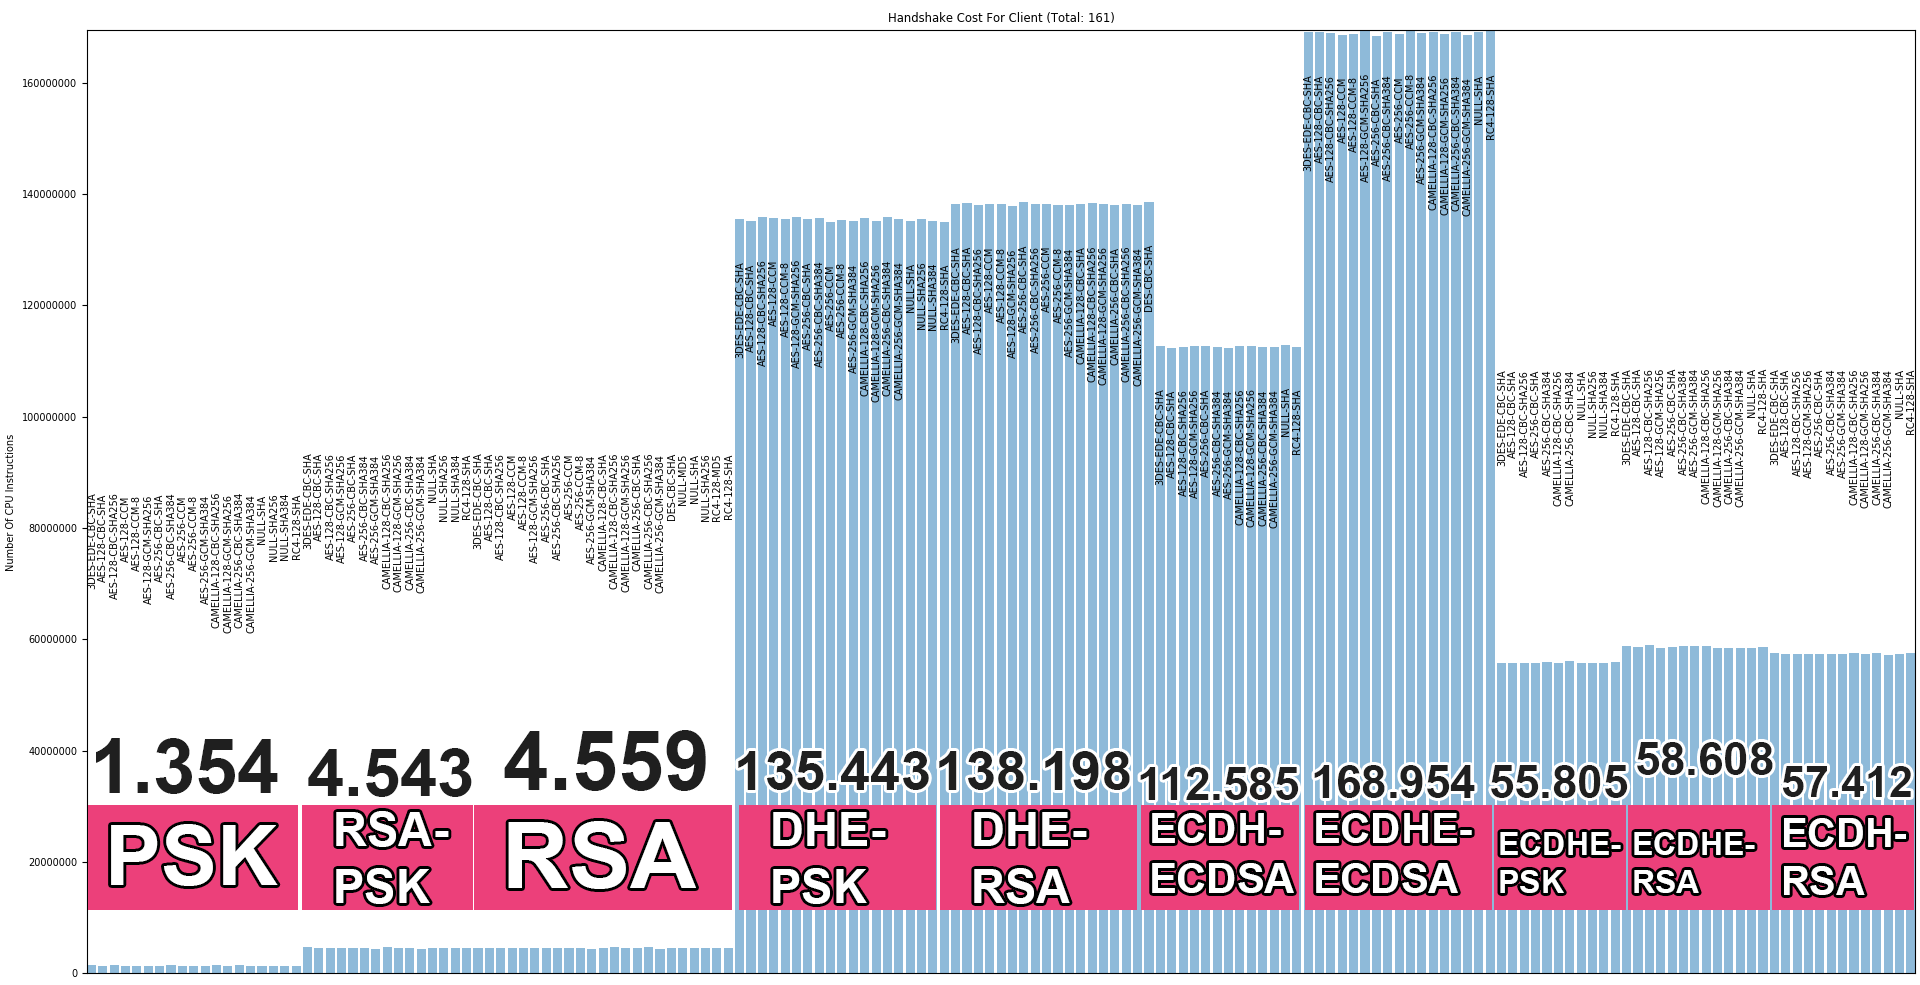
\includegraphics[width=1.0\textwidth]{img/hs_cost_cli.png}
  \centering \caption{\label{fig:hs-all-ciphers-cli} Client handshake cost for all of the $161$ ciphersuites}
\end{figure}

\begin{figure}
  \centering
  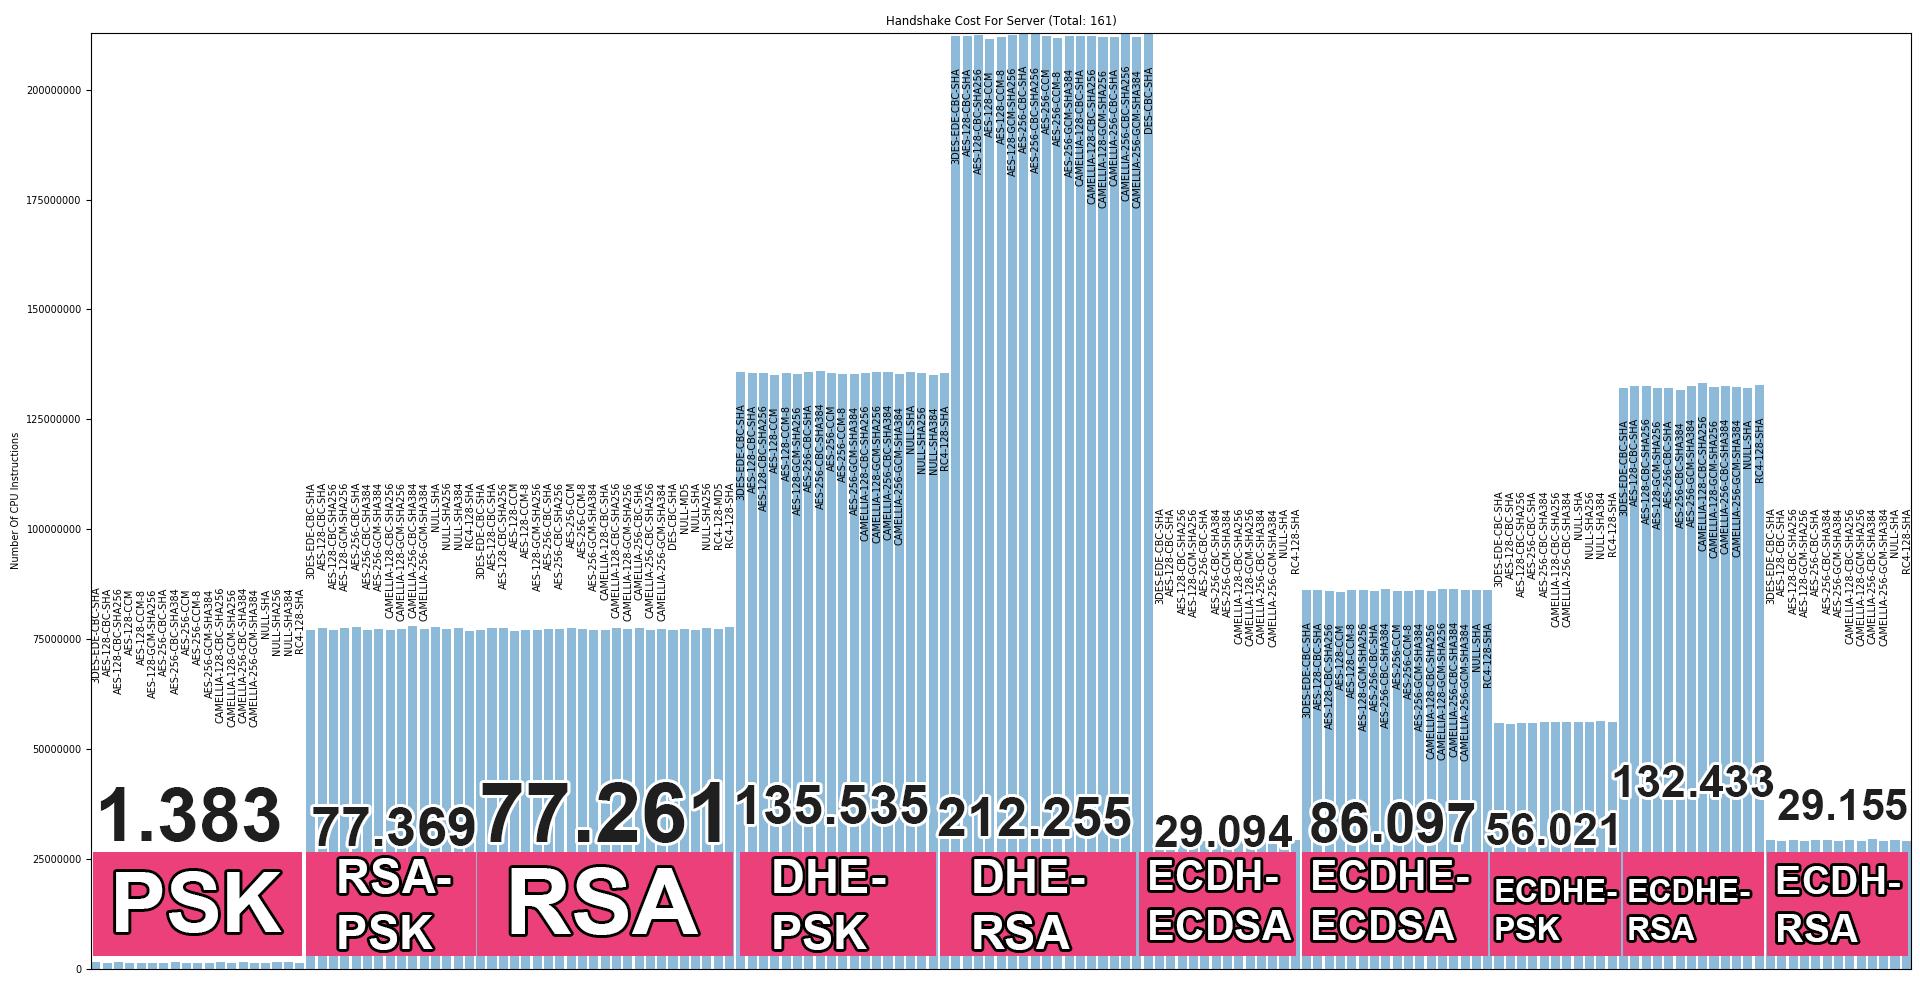
\includegraphics[width=1.0\textwidth]{img/hs_cost_srv.png}
  \centering \caption{\label{fig:hs-all-ciphers-srv} Server handshake cost for all of the $161$ ciphersuites}
\end{figure}

Figures \ref{fig:hs-all-ciphers-cli} and \ref{fig:hs-all-ciphers-srv} depict a graph with the Handshake cost of each one
of the ciphersuites, for the client and the server, respectively. In both graphs, $y$ axis represents the number of
CPU cycles executed. The ciphersuites have been grouped by the key exchange method. Each bar within a key
exchange method group represents a different combination of a symmetric encryption function and a hash function.
The pink rectangles group the ciphersuites by the key exchange method. The numbers at the top of each rectangles indicate the average
number of CPU  cycles, in millions, used to perform the handshake for that key exchange method.
An analysis of both figures shows that there is very little variation in costs within
each key exchange method group. This is due to the fact that most of the resources are spent in authenticating and
generating keying material for \gls{pfs}.

From the analysis of Figures \ref{fig:hs-all-ciphers-cli} and \ref{fig:hs-all-ciphers-srv}, it becomes obvious
that some of the ciphersuites have  much lower handshake costs than the others. For the client, the \textit{PSK} based
ciphersuites are the least and \textit{ECHE-ECDSA} are the most expensive ones. For the server, the \textit{PSK} based
ciphersuites are the least and \textit{DHE-RSA} are the most expensive ones. To make the presented information clearer,
we took the average of the costs of all ciphersuites for each key exchange method. This information is presented in
table \ref{table:hs-all-ciphers-cli-aggr} for the client and in table \ref{table:hs-all-ciphers-srv-aggr} for the server.

\begin{table}[]
\begin{tabular}{cl|l|l|l|l|l|}
\cline{3-7}
\multicolumn{1}{l}{}                                                                        &                          & \multicolumn{2}{c|}{{\ul PFS}}            & \multicolumn{3}{c|}{{\ul No PFS}}                                                                     \\ \cline{2-7}
\multicolumn{1}{l|}{}                                                                       & \cellcolor[HTML]{C0C0C0} & \textbf{DHE}             & \textbf{ECDHE} & \textbf{ECDH}            & \textbf{RSA}                                    & \textbf{X}               \\ \hline
\multicolumn{1}{|c|}{\begin{tabular}[c]{@{}c@{}}Sym\\ Auth\end{tabular}}                    & \textbf{PSK}             & 135.443                  & 55.805         & \cellcolor[HTML]{C0C0C0} & 4.543                                           & 1.354                    \\ \hline
\multicolumn{1}{|c|}{}                                                                      & \textbf{RSA}             & 138.198                  & 58.608         & 57.412                   & \cellcolor[HTML]{C0C0C0}{\color[HTML]{333333} } & 4.559                    \\ \cline{2-7}
\multicolumn{1}{|c|}{\multirow{-2}{*}{\begin{tabular}[c]{@{}c@{}}Asym\\ Auth\end{tabular}}} & \textbf{ECDSA}           & \cellcolor[HTML]{C0C0C0} & 168.954        & 112.585                  & \cellcolor[HTML]{C0C0C0}                        & \cellcolor[HTML]{C0C0C0} \\ \hline
\end{tabular}
\centering
\centering \caption{\label{table:hs-all-ciphers-cli-aggr} Average handshake cost for the client in millions CPU cycles}
\end{table}


\begin{table}[]
\begin{tabular}{cl|l|l|l|l|l|}
\cline{3-7}
\multicolumn{1}{l}{}                                                                        &                          & \multicolumn{2}{c|}{{\ul PFS}}            & \multicolumn{3}{c|}{{\ul No PFS}}                                                                     \\ \cline{2-7}
\multicolumn{1}{l|}{}                                                                       & \cellcolor[HTML]{C0C0C0} & \textbf{DHE}             & \textbf{ECDHE} & \textbf{ECDH}            & \textbf{RSA}                                    & \textbf{X}               \\ \hline
\multicolumn{1}{|c|}{\begin{tabular}[c]{@{}c@{}}Sym\\ Auth\end{tabular}}                    & \textbf{PSK}             & 135.535                  & 56.021         & \cellcolor[HTML]{C0C0C0} & 77.369                                          & 1.383                    \\ \hline
\multicolumn{1}{|c|}{}                                                                      & \textbf{RSA}             & 212.255                  & 132.433        & 29.155                   & \cellcolor[HTML]{C0C0C0}{\color[HTML]{333333} } & 77.261                   \\ \cline{2-7}
\multicolumn{1}{|c|}{\multirow{-2}{*}{\begin{tabular}[c]{@{}c@{}}Asym\\ Auth\end{tabular}}} & \textbf{ECDSA}           & \cellcolor[HTML]{C0C0C0} & 86.097         & 29.094                   & \cellcolor[HTML]{C0C0C0}                        & \cellcolor[HTML]{C0C0C0} \\ \hline
\end{tabular}
\centering
\centering \caption{\label{table:hs-all-ciphers-srv-aggr} Average Handshake cost for the server in millions CPU cycles}
\end{table}

Each row and column intersection in the tables \ref{table:hs-all-ciphers-cli-aggr} and \ref{table:hs-all-ciphers-srv-aggr}
forms a ciphersuite. The rows separate the various authentication algorithms that can be used. The columns separate the
key exchange methods that offer \gls{pfs}, from the ones that don't. Each entry of the table presents the average
number of CPU cycles, in millions. In order to simplify this initial analysis, we are not presenting the standard deviation
values for the averages and are rounding up the results to millions, with $3$ decimal places. In Section \ref{sec:tls-hs-cost} we will present a
more detailed evaluation for all security levels.

\subsubsection{Client}

By analyzing table \ref{table:hs-all-ciphers-cli-aggr}  we can approximate
the costs of the security services of authentication and \gls{pfs} for the client. Even though those values are approximations,
they are very close actual numbers, since they dominate the costs of the Handshake. All of the costs presented in the 
analysis that follows are taken directly from table \ref{table:hs-all-ciphers-cli-aggr} and will be in millions CPU cycles,
rounded to $3$ decimal places.

If \gls{pfs} is used, the cost of the Handshake varies from $55.805$ to $135.443$
million CPU instructions for \gls{psk} based authentication, and from $58.608$ to $168.954$ million CPU cycles for
asymmetric authentication. If the security service of \gls{pfs} is foregone, the cost
of the Handshake varies from $1.354$ to $4.543$ for \gls{psk} based authentication,
and from $4.559$ to $112.585$ for asymmetric authentication.

If we analyze the values in the \textit{ECDHE} column in table \ref{table:hs-all-ciphers-cli-aggr}, thus fixing the
algorithm used to offer \gls{pfs} we can compare the costs of authentication for various algorithms on the client-side.
For example, we can see that \textit{RSA} authentication costs $2.803$  ($58.608 - 55.805$)
more than \gls{psk} authentication and \textit{ECDSA} authentication costs $110.346$ ($168.954 - 58.608$)
million CPU cycles more than
\textit{RSA} authentication. The total cost of using \gls{psk} for authentication can be estimated by looking at the
value in the \textit{PSK} row and \textit{X} column, thus fixing authentication to \textit{PSK} and not using any other
algorithm for key agreement: $1.354$. In fact, we can consider this value to be the overhead of \gls{tls} for the client,
since this is the cost of establishing the most basic \gls{tls} connection available in \textit{mbedTLS 2.7.0}.
In the same manner, the cost of using \textit{RSA} for authentication can
be approximated by taking the value located in row \textit{RSA} and column \textit{X}, thus fixing authentication
to \gls{rsa} and not using any other algorithm for key agreement: $4.559$. Even though we cannot estimate the cost
of using \textit{ECDSA} for authentication directly from the table, we have already seen that \textit{ECDSA} authentication
is $110.346$ more costly than \textit{RSA} authentication. Thus, the cost of using \textit{ECDSA} for authentication
is of $114.905 (4.559+110.346)$ million CPU cycles. When compared, authentication with \gls{rsa} is
$236.7\%$ more expensive than with \gls{psk} and authentication with \gls{ecdsa} is $2420.4\%$ more
expensive than with \gls{rsa}.

Similarly, we can compare the costs of using \gls{dh} vs \gls{ecdh} to provide \gls{pfs}, by
looking at the \gls{psk} (or \gls{rsa}) row, thus fixing the authentication algorithm. Using \textit{DHE} is
$76.638$ ($135.443 - 55.805$) million CPU cycles more $(+142.7\%)$ expensive than using \textit{ECDHE}.
The total cost of \gls{pfs}
using the \gls{ecdh} algorithm can be computed by fixing the \textit{PSK} row (or \gls{rsa} row)
and subtracting the value in the \textit{ECDHE} column from the value in the \textit{X} column. By doing this, we are
fixing the authentication algorithm to \gls{psk} and subtracting the cost of the Handshake when no \gls{pfs} is used,
from the cost of the handshake when \textit{ECDHE} is used to provide \gls{pfs}. Thus, the cost of using \textit{ECDHE}
to provide \gls{pfs} is of $54.451$ million CPU cycles ($55.805-1.354$). Since we already know that \textit{DHE} costs
$76.638$ million CPU cycles more than \textit{ECDHE}, we can compute the cost of using the \textit{DHE} to
provide \gls{pfs}: $131.089 (54.451+76.638)$ million CPU cycles.

\subsubsection{Server}

We will now perform the same analysis for the server by analyzing the table \ref{table:hs-all-ciphers-srv-aggr}. 
Once again, the presented costs will be approximations in
being millions CPU cycles rounded to $3$ decimal places.

If \gls{pfs} is used, the cost of the Handshake varies from $56.021$ to $135.535$
million CPU instructions for \gls{psk} based authentication, and from $86.097$ to $212.255$ million CPU cycles for
asymmetric authentication. If the security service of \gls{pfs} is foregone, the cost
of the Handshake varies from $1.383$  to $77.369$ for \gls{psk} based authentication,
and from $27.094$ to $77.261$ for asymmetric authentication.

If we analyze the values in the \textit{ECDHE} column in table \ref{table:hs-all-ciphers-srv-aggr}, thus fixing the
algorithm used to offer \gls{pfs} we can compare the costs of authentication for various algorithms on the server-side.
For example, we can see that \textit{RSA} authentication costs $76.412$ ($132.433-56.021$) more than \gls{psk}
authentication and \textit{ECDSA} authentication costs $46.336$ ($132.433-86.097$) million CPU cycles less
than \textit{RSA} authentication. The total cost of using \gls{psk} for authentication can be estimated
by looking at the
value in the \textit{PSK} row and \textit{X} column, thus fixing authentication to \textit{PSK} and not using any other
algorithm for key agreement: $1.383$. In fact, we can consider this value to be the overhead of \gls{tls} for the client,
since this is basically the cost of establishing the most basic \gls{tls} connection available in \textit{mbedTLS 2.7.0}.
In the same manner, the cost of using \textit{RSA} for authentication can
be approximated by taking the value located in row \textit{RSA} and column \textit{X}, thus fixing authentication
to \gls{rsa} and not using any other algorithm for key agreement: $77.261$. Even though we cannot estimate the cost
of using \textit{ECDSA} for authentication directly from the table, we have already seen that \textit{ECDSA} authentication
is $46.336$ less costly than \textit{RSA} authentication. Thus, the cost of using \textit{ECDSA} for authentication
is of $30.925 (77.261-46.336)$ million CPU cycles. When compared, authentication with \gls{ecdsa} is
$2136.1\%$ more expensive than with \gls{psk} and authentication with \gls{rsa} is $149.8\%$ more expensive
than with \gls{ecdsa}.

Similarly, we can compare the costs of using \gls{dh} vs \gls{ecdh} to provide \gls{pfs}, by
looking at the \gls{psk} (or \gls{rsa}) row, thus fixing the authentication algorithm. Using \textit{DHE} is
$79.514$ ($135.535 - 56.021$) million CPU cycles more expensive $(+141.9\%)$ than using \textit{ECDHE}. The total cost of \gls{pfs}
using the \gls{ecdh} algorithm can be computed by fixing the \textit{PSK} row (or \gls{rsa} row)
and subtracting the value in the \textit{ECDHE} column from the value in the \textit{X} column. By doing this, we are
fixing the authentication algorithm to \gls{psk} and subtracting the cost of the Handshake when no \gls{pfs} is used,
from the cost of the handshake when \textit{ECDHE} is used to provide \gls{pfs}. Thus, the cost of using \textit{ECDHE}
to provide \gls{pfs} is of $54.638 (56.021-1.383)$ million CPU cycles . Since we already know that \textit{DHE} costs
$79.514$ million CPU cycles more than \textit{ECDHE}, we can compute the cost of using the \textit{DHE} to
provide \gls{pfs}: $134.152 (54.638+79.514)$ million CPU cycles.

\subsubsection{Discussion}

By analyzing at tables \ref{table:hs-all-ciphers-cli-aggr}
and \ref{table:hs-all-ciphers-srv-aggr} it is clear that some ciphersuites are more costly than others. This dissimilarity
can explained by the by fact that different ciphersuites use different security services and different algorithms to
offer those security services. By analyzing the Handshake costs we were able to approximate the costs of the security
services of authentication and \gls{pfs}, as well as of the algorithms used to offer them. This analysis made it clear that the
use or non-use of a security service can have a big impact on the cost of establishing a \gls{tls} connection.

Our analysis showed that \textit{PSK} based ciphersuites are the most efficient ones overall, for both, the client
and the server, thus their popularity in the \gls{iot} environment. Symmetric authentication is, by far,
the least costly one for both peers. For the client, \gls{rsa} is the second least costly authentication and \gls{ecdsa}
is the most costly one of them. For the server, this situation is reversed. The reasons for that will be explained in
Section \ref{sec:asym-algs-analysis}, when we analyze the Handshake costs in detail.

As for the \gls{pfs}, in both cases \textit{ECDHE} is about $1.5$ less costly than \textit{DHE}. This gives us a glimpse
into the benefits of elliptic curve cryptography. The costs of \gls{pfs} are identical for both peers. In the next
section we will analyze both of the security services in more detail.

\subsection{PSK Authentication Cost Analysis} \label{sec:psk-cost-analysis}

In the previous section we compared the costs of different authentication methods by analyzing the total cost of the
Handshake with different ciphersuites. In this section and section \ref{sec:asym-algs-analysis}, we will analyze this 
security service in detail, including the underlying algorithms it. 

In \gls{tls} there are two ways of doing authentication: either by using a \gls{psk} or by using asymmetric cryptography.
If asymmetric cryptography is used, there are two choices for the algorithm: \gls{rsa} or \gls{ecdsa}. We will begin 
with an analysis of \gls{psk} authentication cost in this section and analyze asymmetric authentication costs 
in Section \ref{sec:asym-algs-analysis}.

In the previous section we approximated the cost of \gls{psk} authentication to be $1.354$ million CPU cycles
for the client and $1.383$ million CPU cycles for the server. In reality, this cost is very close to zero, since
both of the parties already have the authentication key. The approximated value is actually the cost of performing the
smallest and least costly handshake in \textit{mbedTLS}.
This value can be considered as the TLS overhead, since it is in essence, the cost of establishing the simplest possible \gls{tls} connection,
without using asymmetric authentication or \gls{pfs}. The majority of those costs are spent in the \gls{prf}, when generating the
shared keying material and in reading/writing the \textit{Finished} message. 

Table \ref{table:hs-key-gen-cost} shows the number of CPU cycles spent in the \gls{prf}
and in computing the \textit{Finished} message for all of the defined security levels.
This number is the average of the runs with each one the $161$ ciphersuites for both of the peers. Thus, it is
an average of $322$ samples. The standard deviation shown in parenthesis.
An analysis of the table shows that the cost of \gls{prf} is almost the same for all security levels. This can be explained by
the fact that it's essentially composed of hashing operations and even if the input size varies
by a few hundred bytes, the total cost does not change by a significant amount.
In \textit{mbedTLS 2.7.0} there are $26$ unique encryption/hash algorithm combinations, $4$ of which use a \textit{NULL} encryption algorithm.
The \textit{Finished} message is the first encrypted message in \gls{tls}. Different encryption algorithms have different
performances. Due to this heterogeneity, the standard deviation is relatively higher for writing and parsing the 
\textit{Finished} message.

\begin{table}[]
\begin{tabular}{|l|l|l|l|l|}
\hline
 \backslashbox{Opeation}{Security\\Level}                       & \textbf{low}   & \textbf{normal} & \textbf{high}  & \textbf{very high} \\ \hline
\textbf{PRF}            & 982957 (14830) & 986854 (19227)  & 992441 (29439) & 1009178 (50185)    \\ \hline
\textbf{Finished Write} & 158717 (22451) & 157912 (23253)  & 156648 (21950) & 158306 (22561)     \\ \hline
\textbf{Finished Parse} & 164680 (23952) & 164984 (26244)  & 163501 (24703) & 164897 (25322)     \\ \hline
\end{tabular}
\centering \caption{\label{table:hs-key-gen-cost} Cost of \gls{prf} and \textit{Finished} message}
\end{table}

The values in table \ref{table:hs-key-gen-cost} remain valid for all key exchange methods, and as we will see,
become insignificant.

\subsection{Asymmetric Algorithms Authentication Cost Analysis} \label{sec:asym-algs-analysis}

If asymmetric cryptography is used for authentication, there are two
choices of algorithms: \gls{rsa} and \gls{ecdsa}. Each one of them has advantages and disadvantages, depending on the
scenario. We will analyze them now.

In \textit{mbedTLS 2.7.0}, there are $31$ ciphersuites that use \gls{rsa} to authenticate ephemeral \gls{dh}/\gls{ecdh} parameters
and $17$ ciphersuites that use \gls{ecdsa} to authenticate ephemeral \gls{dh}/\gls{ecdh} parameters. The metrics from those
ciphersuites can be used to analyze the cost of public and private key operations for both algorithms. Thus, all of the presented
costs for for \gls{rsa} are an average computed from $31$ runs, and for \gls{ecdsa} an average computed from $17$ runs, all from
different ciphersuites.

\gls{rsa} and \gls{ecdsa} have two basic operations: sign and verify. The first one uses the private key, while the
second one the public key. Figure \ref{fig:rsa-ecdsa-sign-ver-total-normal-sl} compares the performance of the algorithm's
operations for the \textbf{normal} security level (\textit{i.e.} $2048$ bit \gls{rsa} key and $256$ bit \gls{ecdsa} key).
The \textit{Total} cost is the sum of the \textit{Sign} and \textit{Verify} costs for the corresponding algorithm.

\begin{figure}
  \centering
  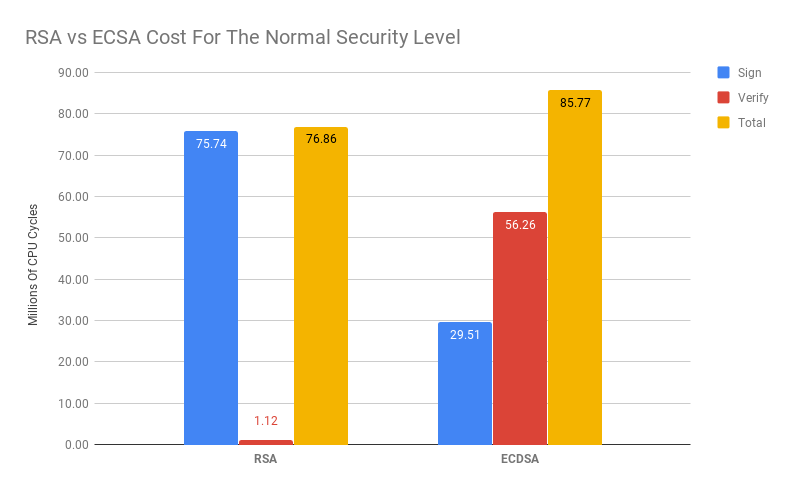
\includegraphics[width=1.0\textwidth]{img/rsa_ecdsa_cost_normal_sl.png}
  \centering \caption{\label{fig:rsa-ecdsa-sign-ver-total-normal-sl} RSA and ECDSA operations cost for normal security level}
\end{figure}

By analyzing the graph, we can can observe two things:

\begin{itemize}
  \item \gls{rsa} is more efficient at performing public key operations, \textit{i.e.} verifying the signature
  \item \gls{ecdsa} is more efficient at performing private key operations, \textit{i.e.} making the signature
\end{itemize}

This holds true for other security levels too, as will be shown further down the text. Let us now analyze each one
of the algorithms and their costs in more detail.

\subsubsection{RSA Cost Analysis}

We have already seen the costs of \gls{rsa} for the \textbf{normal} security level and now we will analyze the
remaining ones. Table \ref{table:rsa-costs-all-sls} shows the number of CPU cycles used
when signing a message with size $20$, $32$ or $48$ bytes and verifying the resulting signature with \gls{rsa} and \gls{ecdsa}.
As already mentioned, the values are an average of $31$ runs for \gls{rsa} and $17$ for \gls{ecdsa}.
The numbers in parenthesis is the standard deviation. All of the values are rounded up to significant digits. The size of the signed message depends on the output size of the
hash function used with the ciphersuite. The cost differences between them are minimal, and for this reason we decided not to separate them.
Table \ref{table:rsa-costs-all-sls-total} presents the sum of the signing and verifying operation cost for \gls{rsa} and \gls{ecdsa}, which we call the \textit{Total} cost.
In out tests, both \gls{rsa} and \gls{ecdsa} signed certificates have signatures over a $32$ byte value (output of \textit{SHA-256}), so
the values in Table \ref{table:rsa-costs-all-sls} apply to those costs too.

Figure \ref{fig:rsa-costs-all-sls} depicts the costs of \gls{rsa} operations graphically. The data is presented in a logarithmic
scale. An analysis of the data shows that the exponential trendline is the one that best fits the cost increase for both, signature creation and
verification. This is a result of modular exponentiation being \gls{rsa}'s core operation. Moreover, for all security levels, the cost of
private key operations is significantly higher than
of the public key ones. The cost of the former also increases more, as the security level raises. For example, there is an increase
of $2145\%$ from the \textit{normal} to \textit{very high} security level for signature creation and of $1102\%$ for signature verification.

This results in a big difference between the cost of creating and verifying signatures, which becomes larger as the security level increases.
For example, at the \textit{normal} security level signature verification is approximately $74.6$ million CPU cycles more expensive,
while at the \textit{very high} security level, this value raises to over $1687$ million, \textit{i.e.} a $2161\%$ increase.

This increase more modest for public key operations, as is shown in Figure \ref{fig:rsa-pub-priv-cost-increase}.
The percentages show the relative cost increase from the previous security level. For example, creating an \gls{rsa} signature costs
$268.4\%$ more at \textit{normal} than at \textit{low} security level. For all operations, the cost increase is exponential.
The consequences of the exponential cost increase are shown in table \ref{table:rsa-absolute-cost-increase}, which presents this relative increase
in terms of absolute values. The numbers are increasing, with the signature creation increase being significantly larger
than the signature verification one. An analysis Figure \ref{fig:rsa-pub-priv-cost-increase}
explains the difference between the costs of private and public key operations. As the security level increases, the relative cost
increase is larger for signing than for verifying. On average, the signing operation cost increase from one security level to another
is about $1.5$ larger than the verifying one. This has a cumulative effect: the constantly larger value increases even more.
This is shown graphically in Figure \ref{fig:rsa-ecdsa-pub-priv-ratio}, which for \gls{rsa}, presents the ratio between the cost of private and
public key operations. As the security level increases, the value becomes larger. The fact that the signing operation dominates the total cost
can also be seen graphically in Figure \ref{fig:rsa-pub-priv-cost-increase}. The \textit{Total} cost increase line is very close to the
\textit{RSA Sign} cost increase line, in fact, they're almost identical. On average, the \textit{Total} cost increase is only $1.4\%$ smaller
than the signing operation cost increase.

\begin{figure}
  \centering
  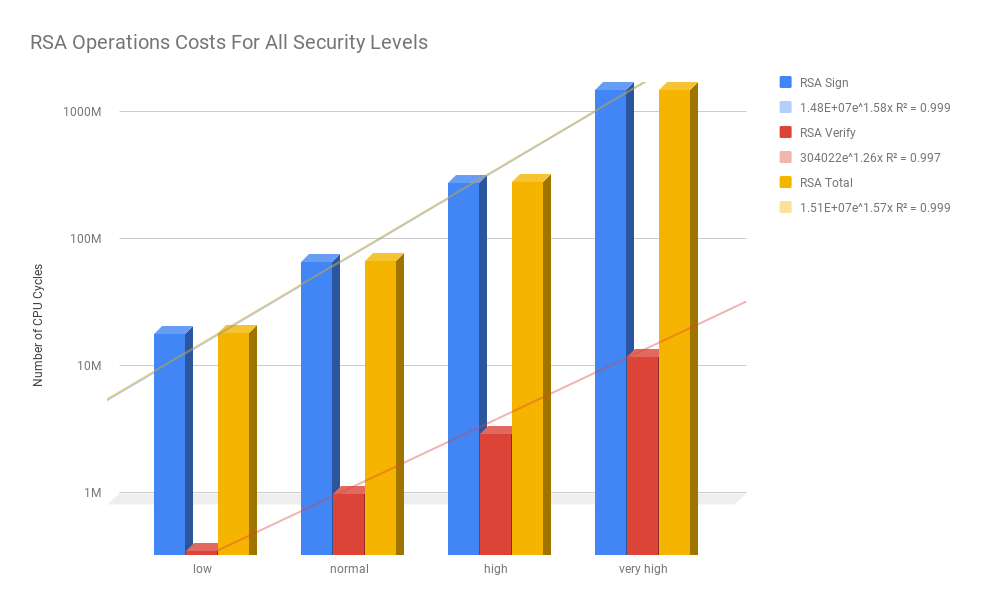
\includegraphics[width=1.0\textwidth]{img/rsa_cost_all_sls.png}
  \centering \caption{\label{fig:rsa-costs-all-sls} RSA operations costs for all security levels (logarithmic scale)}
\end{figure}

\begin{figure}
  \centering
  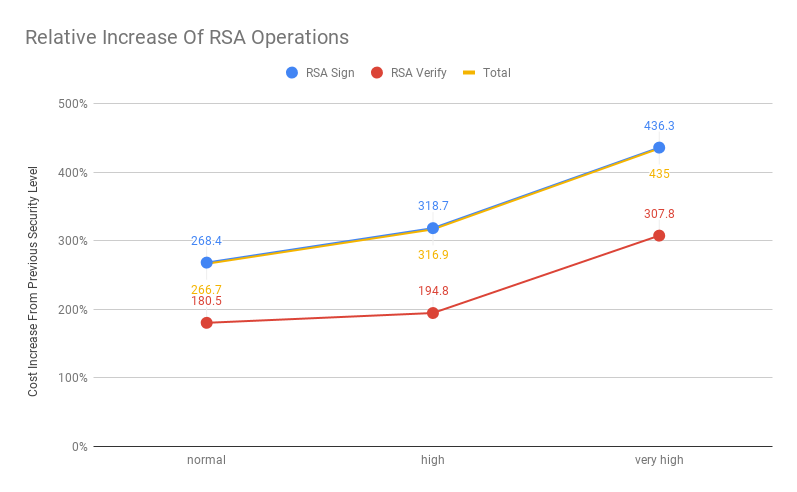
\includegraphics[width=1.0\textwidth]{img/rsa_relative_increase.png}
  \centering \caption{\label{fig:rsa-pub-priv-cost-increase} Relative increase of RSA operation costs}
\end{figure}

\begin{figure}
  \centering
  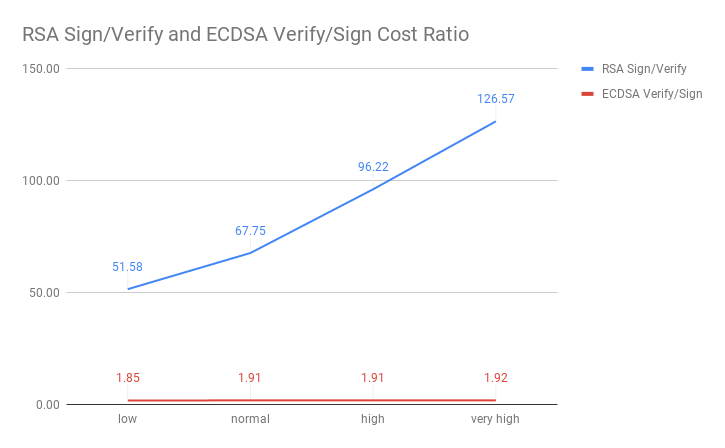
\includegraphics[width=1.0\textwidth]{img/rsa_ecdsa_operation_ratio.png}
  \centering \caption{\label{fig:rsa-ecdsa-pub-priv-ratio} Ratio between the most and the least costly operation for RSA and ECDSA}
\end{figure}

The reason for the discrepancy between the cost of public and private key operations has to do with an optimization
in the choice of the keys. \gls{rsa}'s public keys are deliberately chosen to have a small public exponent, such as $e=65537$. This is considered as a
sensible compromise, since it is famously known to be prime, large enough to avoid the attacks to which
small exponents make RSA vulnerable, and can be computed extremely quickly on binary computers \cite{boneh2002fast}\cite{muir2006seifert}.
A smaller exponent leads to less exponentiation operations, thus better performance. For this reason, public
key operations with \gls{rsa} are faster than private key ones.

\subsubsection{ECDSA Cost Analysis}

After analyzing the costs of \gls{rsa}, we will now perform a similar analysis for \gls{ecdsa}. Figure \ref{fig:ecdsa-costs-all-sls}
shows the costs of \gls{ecdsa} operations graphically. The values are taken from Table \ref{table:rsa-costs-all-sls}. Unlike in \gls{rsa},
in \gls{ecdsa} the private key operation is the least costly one. Figure \ref{fig:rsa-ecdsa-pub-priv-ratio} shows this ratio for both,
\gls{rsa} and \gls{ecdsa}. Besides the ratio being a lot smaller for \gls{ecdsa}, it varies very little. This means, that no matter
the security level, \gls{ecdsa} signature verification will always be about $2$ times more costly than signature creation.

As it is shown in figure \ref{fig:ecdsa-costs-all-sls}, a logarithmic trendline is the one that best fits the cost increase for both,
signature creation and verification.
Figure \ref{fig:ecdsa-relative-cost-incerase} shows the relative cost increase of of \gls{ecdsa}'s operations. The percentages
are the relative cost increase from the previous security level. There are two major differences from \gls{rsa}. First, the relative cost increase
of signature creation and verification is very similar. Consequently, the same is true for the total cost increase. This can be confirmed
graphically in Figure \ref{fig:ecdsa-relative-cost-incerase}, where all of the lines are
close one to another. As a result, even with the increase of security level, none of the operations will dominate in cost as much as it happens
in \gls{rsa}. Second, as the security level increases, the cost increase from the previous security level becomes smaller. In fact, after the
\textbf{high} security level, the absolute cost increase starts decreasing as well. We can see this in table \ref{table:ecdsa-absolute-cost-increase}.
This is a consequence of the cost increase being logarithmic, which is a result of \gls{ecdsa}'s core mathematical operation being
multiplication of a scalar by a point on the curve. Although not presented here, this trend continues for higher security levels.
Those properties of \gls{ecdsa} makes the security level increase more manageable. It's not as costly to increase the security level for
\gls{ecdsa} as it for \gls{rsa}.

\begin{figure}
  \centering
  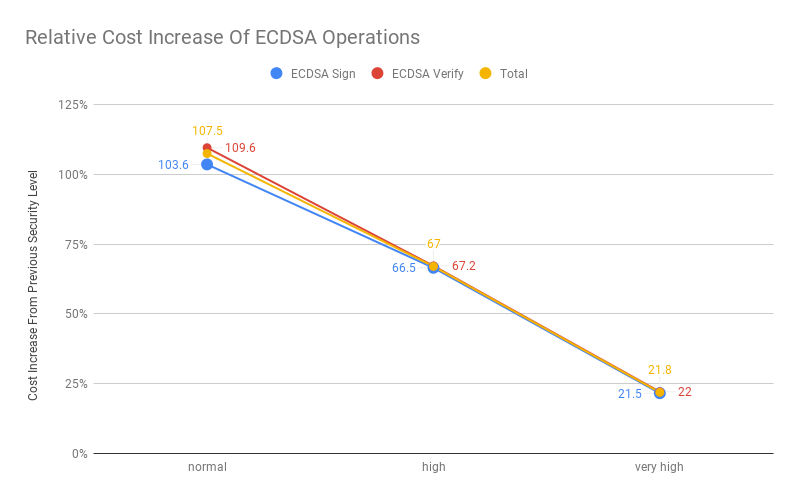
\includegraphics[width=1.0\textwidth]{img/ecdsa_realtive_cost_increase.png}
  \centering \caption{\label{fig:ecdsa-relative-cost-incerase} Relative increase of ECDSA operations cost}
\end{figure}

\begin{figure}
  \centering
  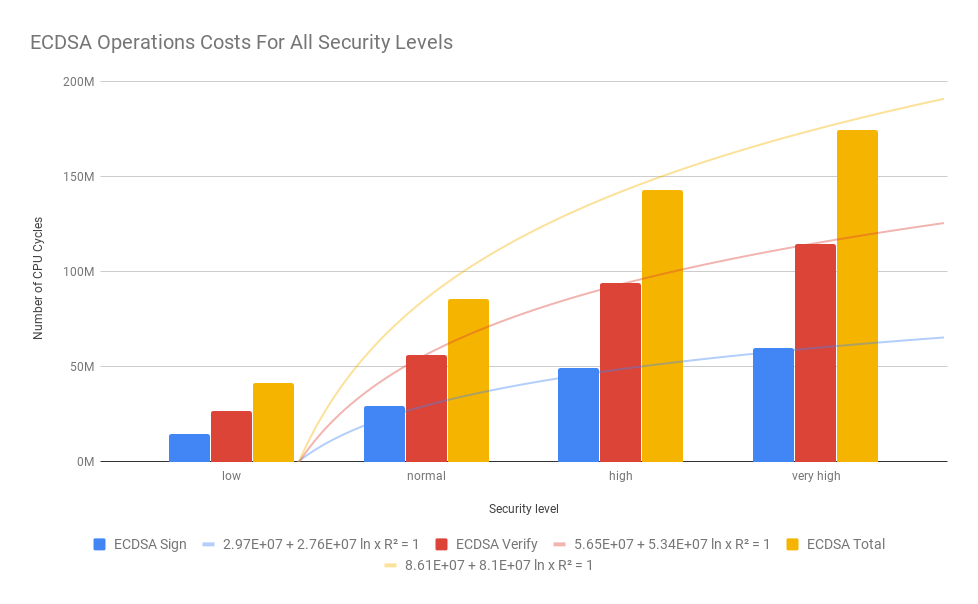
\includegraphics[width=1.0\textwidth]{img/ecdsa_cost_all_sls.png}
  \centering \caption{\label{fig:ecdsa-costs-all-sls} ECDSA costs for all security levels}
\end{figure}

In the previous subsection we have described an optimization in the choice of keys for \gls{rsa}. There are no such optimizations
for \gls{ecdsa}. For this reason, it is expected that the cost of both operations will increase in similar proportion. The non-optimized
key (private for \gls{rsa}, private and public for \gls{ecdsa}) operation cost increase is a lot smaller for \gls{ecdsa}. This can be
explained by the fact that smaller keys are used in \gls{ecdsa}, as we have already seen in Table \ref{table:ecc-key-sizes},
and is a big advantage of \gls{ecc}.

\subsubsection{RSA vs ECDSA} \label{sec:rsa-vs-ecdsa}

After having analyzed the costs of \gls{rsa} and \gls{ecdsa}, we will now compare both and draw some conclusions. The answer to the
question of which one of algorithms is less costly will vary depending on the security level and the operation. Figure \ref{fig:ecdsa-rsa-costs-all}
shows the costs of both, \gls{rsa}'s and \gls{ecdsa}'s operations. The data is presented in logarithmic scale. Since for \gls{rsa} most
of the \textit{Total} cost comes from the signature creation operation, those two lines overlap in the graph.

\begin{figure}
  \centering
  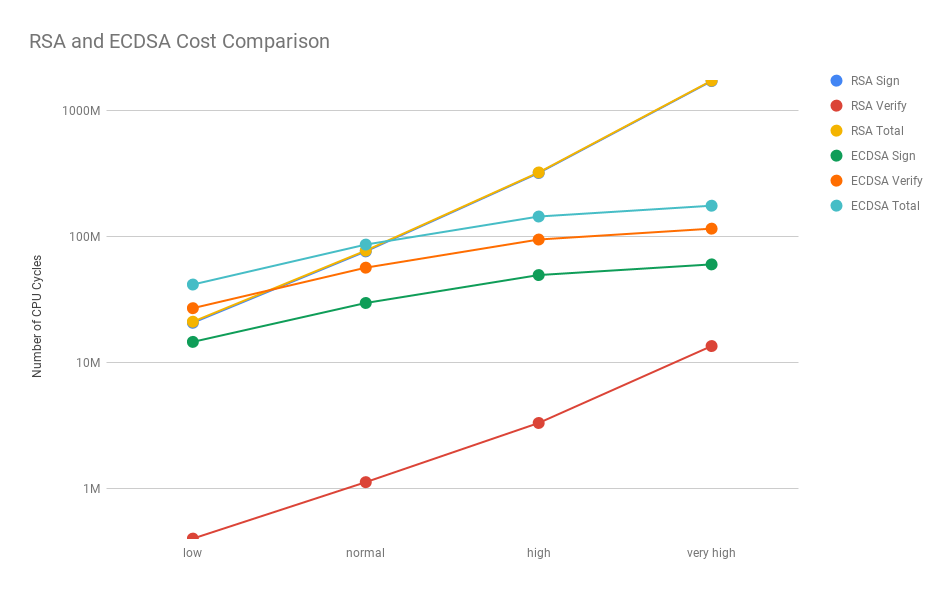
\includegraphics[width=1.0\textwidth]{img/rsa_ecdsa_costs_all.png}
  \centering \caption{\label{fig:ecdsa-rsa-costs-all} RSA and ECDSA cost comparison}
\end{figure}

By analyzing Figure \ref{fig:ecdsa-rsa-costs-all}, we can answer the question of \textit{Which algorithm is less costly?}:

\begin{itemize}
  \item \gls{rsa} is always less costly at signature verification
  \item \gls{ecdsa} is always less costly at signature creation
  \item \gls{rsa}'s cost increase is exponential
  \item \gls{ecdsa}'s cost increase is logarithmic
  \item Total cost of \gls{rsa} is smaller for the \textit{low} and \textit{normal} security levels
  \item Total cost of \gls{ecdsa} is smaller for the \textit{high} and \textit{very high} security levels
\end{itemize}

By analyzing figures \ref{fig:rsa-pub-priv-cost-increase} and \ref{fig:ecdsa-relative-cost-incerase}, and tables \ref{table:rsa-absolute-cost-increase} and
\ref{table:ecdsa-absolute-cost-increase} which show the relative and absolute cost increases for \gls{rsa} and \gls{ecdsa} operations,
we can see that as the security level increases, the cost increase of \gls{rsa} operations from the previous security level always always increases, 
while after the \textbf{normal} security level, the cost increase of \gls{ecdsa} operations from the previous security level starts decreasing.
Although not presented here,  our tests show that this trend holds true
for higher security levels as well. This is a consequence of \gls{rsa} having an exponential cost increase, while \gls{ecdsa} a logarithmic one.
For this reason, it is safe to say that for security levels higher than the ones that we defined, \gls{ecdsa} would be the preferred choice.
\gls{rsa}'s cost increases exponentially due to the mathematical operation at the algorithm's core: modular exponentiation. Similarly, the cost
increase in \gls{ecdsa} is logarithmic, due its \gls{ecc} properties: the base mathematical operation is multiplication of a scalar by a point on the
curve.

So which algorithm should be used for each security level? The answer to this question is not straightforward and will depend on the environment.
For example, if the scenario is a constrained client and a non-constrained server, \gls{rsa} would be the least costly choice. If, on the
other hand, the server is the constrained node, \gls{ecdsa} would be the least costly algorithm. If both of the nodes are
constrained minimizing \textit{Total} cost is the goal, thus \gls{rsa} would be the least costly choice for the \textit{low} and 
\textit{normal} security levels, and \gls{ecdsa} for the remaining ones. If the objective is to have the costs for both peers as similar as 
possible, \gls{ecdsa} is the algorithm to use.

This information can also be used to make
certificate choices for mutual authentication scenarios, \textit{i.e.} when both, the client and the server authenticate one to another.
For example, if only one of the nodes is constrained, an \gls{rsa}-singed certificate from the non-constrained node and an \gls{ecdsa}-signed
certificate from the constrained node would minimize the costs for the constrained node. If both of the nodes are constrained, then the
choice of the least costly algorithm will be guided by the \textit{Total} cost: \gls{rsa} for the \textit{low} and \textit{normal}
security levels and \gls{ecdsa} for the \textit{high} and \textit{very high} security levels.

\subsubsection{The Cost Of Authentication in TLS} \label{sec:auth-cost-in-tls}

Having analyzed the costs of the algorithms that can be used for authentication, we will now describe the cost of this security service
for each one of the ciphersuites for the client and the server. Table \ref{table:tls-auth-cost-client} shows authentication costs for each
ciphersuite for the client. Table \ref{table:tls-auth-cost-server} shows the same information for the server. Each row specifies a key
exchange method and each column the security level.

\begin{figure}
  \centering
  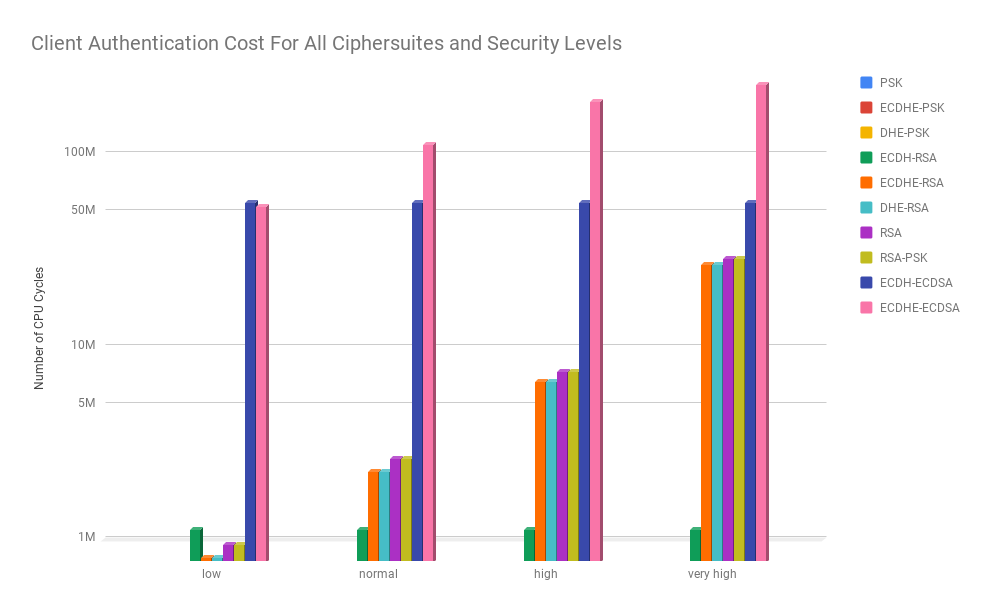
\includegraphics[width=1.0\textwidth]{img/tls-client-auth-cost.png}
  \centering \caption{\label{fig:tls-auth-cost-client} Client authentication cost (logarithmic scale)}
\end{figure}

\begin{figure}
  \centering
  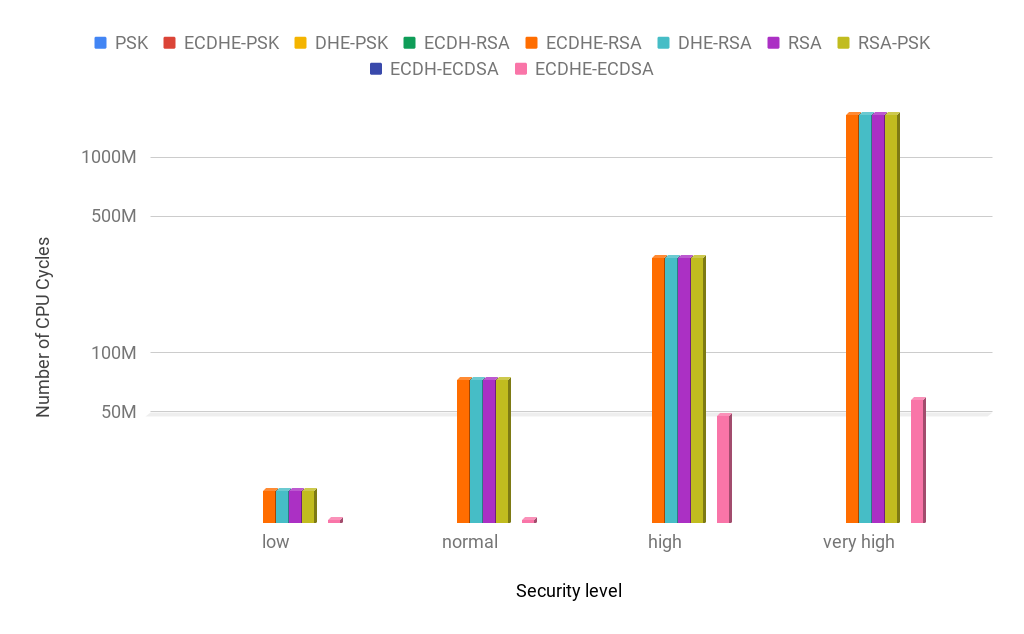
\includegraphics[width=1.0\textwidth]{img/tls-server-auth-cost.png}
  \centering \caption{\label{fig:tls-auth-cost-server} Server authentication cost (logarithmic scale)}
\end{figure}


Figures \ref{fig:tls-auth-cost-client} and \ref{fig:tls-auth-cost-server} are a graphical representation of tables \ref{table:tls-auth-cost-client} and \ref{table:tls-auth-cost-server},
respectively. In both of the figures, the data is presented in logarithmic scale. By looking at the graphs, it becomes evident that the some ciphersuites can be grouped together by authentication cost.
For the client, those groups are:

\begin{enumerate}
  \item \textit{PSK}, \textit{ECDHE-PSK}, \textit{DHE-PSK}
  \item \textit{ECDH-RSA}
  \item \textit{ECDHE-RSA}, \textit{DHE-RSA}
  \item \textit{RSA}, \textit{RSA-PSK}
  \item \textit{ECHD-ECDSA}
  \item \textit{ECHDE-ECDSA}
\end{enumerate}

For the server, those groups are:

\begin{enumerate}
  \item \textit{PSK}, \textit{ECDHE-PSK}, \textit{DHE-PSK}, \textit{ECDH-RSA}, \textit{ECDH-ECDSA}
  \item \textit{ECHDE-ECDSA}
  \item \textit{ECDHE-RSA}, \textit{DHE-RSA}
  \item \textit{RSA}, \textit{RSA-PSK}
\end{enumerate}

Inside every group, the authentication cost is the same, regardless of the security level. Group numbers are ordered in ascending cost order, with Group $1$
being the least costly one, Group $2$ the second least costly one, and so on. All ciphersuites in the same group share a common set of operations that
are performed to provide authentication. We will discuss what those operations are further down in the text. Each ciphersuite uses either \gls{psk},
\gls{rsa} or \gls{ecdsa} for authentication. If only \gls{psk} is used for authentication, the cost of authentication is $0$. This is the case of Group
$1$ for the client and the server. At the end of the previous section we discussed which algorithm, \gls{rsa} or \gls{ecdsa} would be the least costly
choice. An analysis of authentication costs in \gls{tls} goes in hand with that discussion. By analyzing tables 
\ref{table:tls-auth-cost-client} and \ref{table:tls-auth-cost-server}, and figures \ref{fig:tls-auth-cost-client} and 
\ref{fig:tls-auth-cost-server}, we can see that the cheapest choice for the client is \gls{rsa} and for the
server is \gls{ecdsa}. Similarly, for \gls{pfs} enabled ciphersuites, if the goal is to make the cost distribution as even as possible among 
the peers, \gls{ecdsa} is the preferred choice. Having presented the costs of authentication for various key exchange methods 
and made a high-level analysis, we will now go into more detail and justify each value.

In \gls{tls} it hard to talk about the cost of authentication without  talking about \gls{pfs}. If a \gls{pfs}-enabled
ciphersuite is used, an additional piece of information is authenticated in all non-\gls{psk} ciphersuites: the \textit{ServerKeyExchange} message.
This message contains a signature over the hash of the public \textit{(EC)DH parameters}. This has an implication on the signature creation cost
for the server and signature verification cost for the client. All non-\gls{psk} key exchange methods which begin with either
\textit{ECDHE} or \textit{DHE} incur in that extra cost.  We can use the values for the appropriate security level from table
\ref{table:rsa-costs-all-sls} to estimate them.

All \gls{rsa} server certificates are signed with a $2048$ bit \gls{rsa} key and all \gls{ecdsa} certificates
are signed with a $256$ bit \gls{ecdsa} key. This signature is made over an \textit{SHA-256} hash, which has an output size of $32$ bytes.
Thus, we can use the values from the \textit{normal} security level from table \ref{table:rsa-costs-all-sls} to compute the certificate signature
verification costs.

In \textit{RSA} and \textit{RSA-PSK} ciphersuites, the client uses the \textit{PKCS\#1 v2.1 RSAES-PKCS1\-V1\_5\-ENCRYPT}\cite{RFC3447}
encryption scheme to encrypt  the $48$ byte premaster secret. The server uses the corresponding \textit{PKCS\#1 v2.1 RSAES-PKCS1\-V1\_5\-DECRYPT}\cite{RFC3447}
decryption scheme to decrypt it. The costs of those operations are higher than of the regular sign/verify ones, due to extra steps performed.
Thus, to compute the authentication cost for those ciphersuites, in addition the the values from table \ref{table:rsa-costs-all-sls}, the ones
from table \ref{table:pkcs-cost} will also be used. In \textit{mbedTLS 2.7.0}, there are a total of
$38$ ciphersuites that use the \textit{PKCS\#1 v2.1} scheme as part of the authentication process: $23$
\textit{RSA} ciphersuites and $15$ \textit{RSA-PSK} ciphersuites. The values in table \ref{table:pkcs-cost} are an average
of $38$ runs: one for each ciphersuite. The numbers in parenthesis is the standard deviation.

\begin{table}[]
  \resizebox{\textwidth}{!}{
  \begin{tabular}{|l|l|l|l|l|}
  \hline
   \backslashbox{Operation}{Security\\Level}                & \textbf{low}      & \textbf{normal}   & \textbf{high}      & \textbf{very high}   \\ \hline
  \textbf{Encrypt} & 542291 (836)      & 1504367 (2012)    & 4167693 (2866)     & 15280266 (3748)      \\ \hline
  \textbf{Decrypt} & 20362831 (125590) & 75129504 (252921) & 314975365 (676291) & 1691976601 (2015526) \\ \hline
  \end{tabular}}
  \centering \caption{\label{table:pkcs-cost} Cost of using \textit{PKCS\#1 V2.1 RSAES-PKCS1-v1\_5} encryption and decryption schemes with various security levels}
  \end{table}

The encryption operation uses the server's public key and the decryption operation the corresponding private key. Thus, as expected,
decryption is more costly than the encryption and both of the values increase, as the security level increases.

In order to authenticate, the client and the server perform different steps, depending on the ciphersuite. More specifically:

\begin{itemize}
  \item  in \textit{PSK}, \textit{DHE-PSK} and \textit{ECDHE-PSK} the authentication is done exclusively through the pre-shared secret, without any
  operations, thus the authentication cost is $0$.
  \item in \textit{RSA} and \textit{RSA-PSK} the client has to verify the server's \gls{rsa}-signed certificate and encrypt the premaster secret with
  the server's public \gls{rsa} key, while the server has to decrypt the premaster secret with the corresponding private key.
  \item in \textit{ECDH-RSA} ciphersuites, the client has to verify the server's \gls{rsa}-signed certificate and the server does not
  need to perform any operations.
  \item in \textit{ECDH-ECDSA} ciphersuites, the client has to verify the server's \gls{ecdsa}-signed certificate and the server does not
  need to perform any operations.
  \item in \textit{ECHDE-RSA} and \textit{DHE-RSA} ciphersuites the client has to verify the server's \gls{rsa}-signed certificate and
  the \textit{(EC)DH} \gls{rsa}-signed parameters, while the server has to perform an \gls{rsa} signature over the hash of \textit{(EC)DH} parameters.
  \item in \textit{ECHDE-ECDSA} ciphersuites the client has to verify the server's \gls{ecdsa}-signed certificate and
  the \textit{(EC)DH} \gls{ecdsa}-signed parameters, while the server has to perform an \gls{ecdsa} signature over the hash of \textit{(EC)DH} parameters.
\end{itemize}

In order to compute the authentication cost for each peer, we use the values from tables \ref{table:rsa-costs-all-sls} and \ref{table:pkcs-cost},
sum them up according to the steps described above. For example, when an \textit{ECDHE-ECDSA} ciphersuite is used at the \textit{normal} security level,
the client verifies two \gls{ecdsa} signatures: one from the parsed server's certificate
and one from the \textit{ServerKeyExchange} message, while the server only performs a signature over the \textit{ECDHE} parameters.
Thus, the authentication cost for the client will be $56260702+56260702=112521404$ and for the server $29512991$. Similarly, when an \textit{RSA} or
\textit{RSA-PSK} ciphersuite is used at the \textit{normal} security level, the client will verify the \gls{rsa} signature in the server's certificate
and perform a \textit{PKCS\#1 v2.1 RSAES-PKCS1\-V1\_5} encryption, while the server will only need to perform a
\textit{PKCS\#1 v2.1 RSAES-PKCS1\-V1\_5} decryption. Thus, the authentication cost for the client will be $1117868+1504367=2622235$ and for the server
$75129504$. The remaining entries in tables \ref{table:tls-auth-cost-client} and \ref{table:tls-auth-cost-server} are computed in a similar manner.
It is important to remember that independently of the security level, in our evaluation the server's certificates are always signed with either a 
$2048$ bit \gls{rsa} keys or $256$ bit \gls{ecdsa} keys. Thus, for the certificate signature verification cost on the client side, 
the values from the \textit{normal} security row of table \ref{table:rsa-costs-all-sls} are used.

Since in our evaluated scenario only the server authenticates, tables \ref{table:tls-auth-cost-client} and \ref{table:tls-auth-cost-server}
are non-identical. If mutual authentication was used (\textit{i.e.} with both, the client and server authenticating one to another), there would be
an additional cost of creating a signature for the client and of verifying the corresponding signature for the server.

\subsection{Perfect Forward Secrecy Cost Analysis} \label{sec:pfs-costs}

In \gls{tls} there are two ways of achieving \gls{pfs}: either by using the \gls{dh} algorithm or its \gls{ecc} counterpart \gls{ecdh}.
In section \ref{sec:ss-overview} we estimated the cost of \gls{pfs} and compared the two methods of achieving it by analyzing the total cost of the
Handshake with different ciphersuites. In this section, we will analyze this security service in detail, including the underlying algorithms.
In \gls{dh} and \gls{ecdh} the same basic operations are performed by each peer in sequence: generate a public/private keypair, exchange the public values
and derive the shared secret.

In \textit{mbedTLS 2.7.0} there are a total of $78$ ciphersuites that offer \gls{pfs}. $41$ of them use the \gls{ecdh} algorithm and $37$ of them use
the \gls{dh} algorithm. There are also $26$ ciphersuites that do not offer \gls{pfs}, but still use the \gls{ecdh} algorithm. The metrics obtained from the
Handshake analysis with those ciphersuites can be used to analyze the cost of the algorithms. Since the operations performed at the client and
the server side are identical, we do not need to present two separate analysis, like we did throughout Section \ref{sec:asym-algs-analysis}.
Moreover for \textit{ECDHE} and \textit{DHE}, we can analyze the metrics from both  of the peers in conjunction, thus doubling the sample size.
As for \textit{ECDH} ciphersuites, we can use the client-side results to analyze the cost of all \gls{ecdh} operations and the server-side results
to analyze the cost of the shared \gls{ecdh} secret generation operation.

Thus, all the presented cost values for \gls{ecdh}'s ephemeral key pair generation are an average computed from $108$ runs ($41$ from each
peer's \gls{pfs} ciphersuites and $26$ from client's non-\gls{pfs} ciphersuites),
and for the shared secret generation an average of $134$ runs ($41$ from each peer's \gls{pfs} ciphersuites and $26$ from each peer's non-\gls{pfs}
ciphersuites). For the \gls{dh} algorithm, the average for both operations is computed from $74$ runs ($37$ from each peer).

\begin{figure}
  \centering
  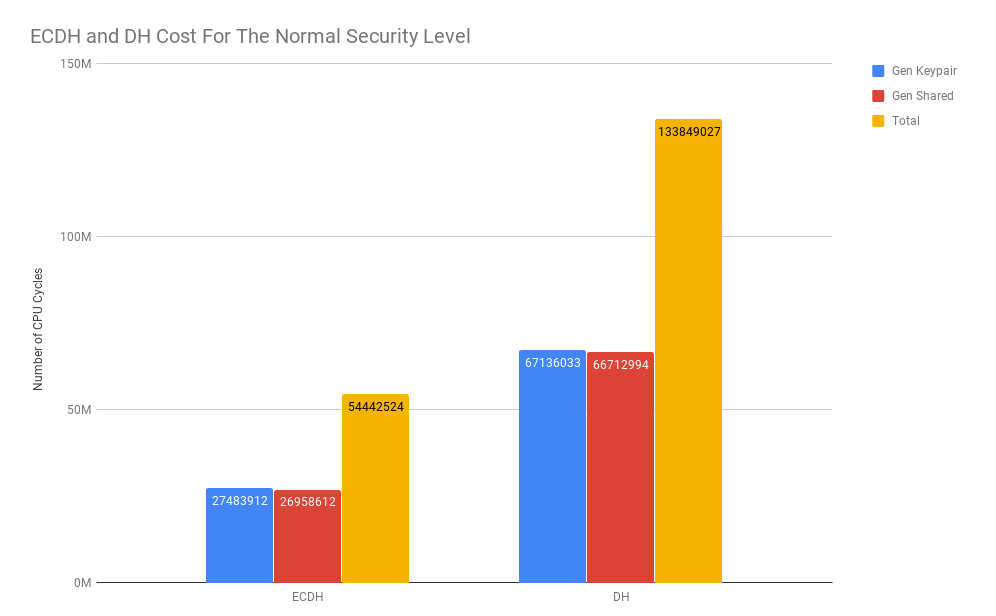
\includegraphics[width=1.0\textwidth]{img/ecdh-dh-cost-normal-sl.png}
  \centering \caption{\label{fig:ecdh-dh-cost-normal-sl} ECDH and DH operations cost for normal security level}
\end{figure}

Figure \ref{fig:ecdh-dh-cost-normal-sl} compares the cost of \gls{ecdh}'s and \gls{dh}'s operations for the \textbf{normal} security level.
The total cost is the of the keypair and shared secret generation values for the corresponding algorithm. By analyzing the graph, we can can
observe two things:

\begin{itemize}
  \item \gls{ecdh} is less costly than \gls{dh}
  \item for both algorithms, the costs of generating the key pair and the shared secret are very similar.
\end{itemize}

The first observation is true starting from the \textbf{normal} security level and onwards.
The fact that for each algorithm the cost of generating the public/private keypair is very similar to the cost of generating secret is not a coincidence.
\gls{ecdh} and \gls{dh} use different mathematical operations, but for each algorithm, those operations are the same for the operations of keypair
shared secret generation. Thus, it is expected for the cost of both steps being almost identical. We will now analyze each one of the algorithms and
their costs in more detail.

\subsubsection{ECDH Cost Analysis}

In \gls{ecdh}, two basic operations are performed by each peer: first, a public/private \gls{ecc} keypair is generated, followed by generation of
the shared secret. The resulting shared secret will be a 2D $(x,y)$ coordinate on the curve. In \gls{tls} the $y$ value is discarded and $x$ is
used as the preshared secret. Computing the private key is cheap, since it is just a randomly generated number. The costly part is the computation of
the public key and the shared secret, since for both it involves multiplications of a scalar by a point on the elliptic curve.

We have already seen the costs of \gls{ecdh} for the \textbf{normal} security level and now we will analyze the remaining ones. Table
\ref{table:ecdh-dh-costs-all-sls} shows the number of CPU cycles for each \gls{ecdh} and \gls{dh} operation. As already mentioned, the values are
an average of $108$ runs for the \gls{ecdh}'s key generation, $134$ runs for \gls{ecdh}'s shared secret generation and of $34$ runs for both of \gls{dh}'s
operations. The numbers presented in parenthesis is the standard deviation. All of the values are rounded up to significant digits.
Table \ref{table:ecdh-dh-costs-total-all-sls} presents the sum of keypair and shared secret generation operations for for \gls{ecdh} and \gls{dh},
which we call the \textit{Total} cost. For both algorithms, the cost of generating the private key is less than $1\%$ of the keypair generation operation.
This is expected as the private key is just a randomly generated number, with size specific to the elliptic curve's group.

Figure \ref{fig:ecdh-costs-all-sls} depicts the cost of \gls{ecdh} operations graphically. For all security levels the total cost is almost
evenly divided between the keypair and the shared secret generation. This is justified by the fact that the underlying mathematical operation is
the same when generating the public/private keys and the shared secret: multiplications of a scalar by a point on the curve. An analysis of the figure
also shows that a logarithmic trendline is the one that best fits the cost increase for all operations.

\begin{figure}
  \centering
  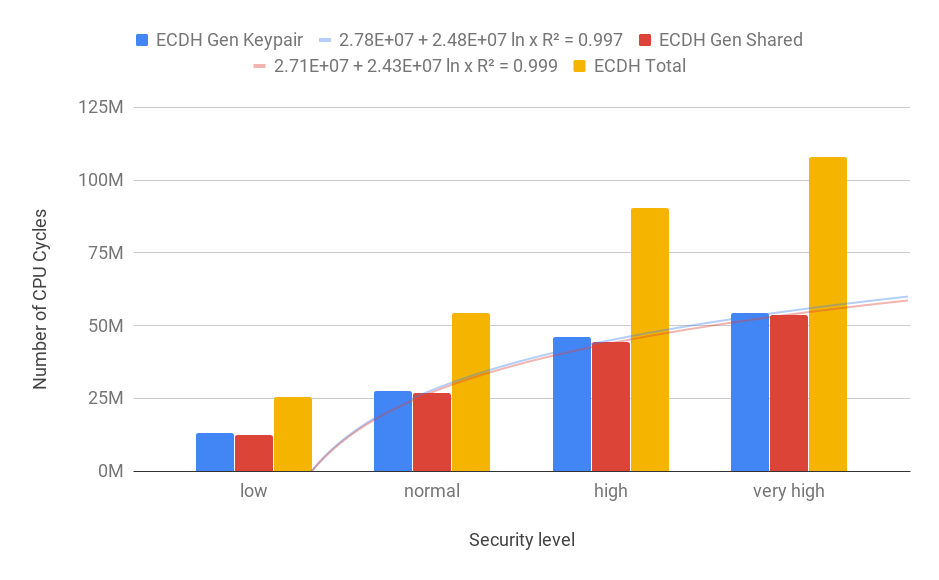
\includegraphics[width=1.0\textwidth]{img/ecdh_cost_all_sls.png}
  \centering \caption{\label{fig:ecdh-costs-all-sls} ECDH operations costs for all security levels}
\end{figure}

Figure \ref{fig:ecdh-dh-relative-cost-increase} shows the relative cost increase of \gls{ecdh} operations from the previous security.
The cost increase of generating the keypair, the shared secret, and consequently of their sum, is very similar, thus the $3$ lines overlap.
As expected, the total relative cost increase represents the average of the values of keypair and shared secret generation relative increase.
By analyzing the graph, we can see  that as the security level increases, the cost increase  from the previous security
level becomes smaller. The effect decrease on the absolute cost increase can be seen in table \ref{table:ecdh-absolute-cost-increase}.
This table shows the absolute increase in the number of CPU cycles from
the previous security level. What can be clearly seen in this table is that after the \textbf{high} security level, the absolute cost increase starts
going down. Although not presented here, those trends continue for higher security levels.

There is a striking resemblance between the cost analysis of \gls{ecdh} and \gls{ecdsa}. In both algorithms, the cost increase is logarithmic.
In fact, the percentages for \gls{ecdsa} and \gls{ecdh} in figures \ref{fig:ecdsa-relative-cost-incerase}
and \ref{fig:ecdh-dh-relative-cost-increase}, we can see that the numbers are very similar. This similarity also reflects in the
trend that can be seen in tables \ref{table:ecdsa-absolute-cost-increase} and \ref{table:ecdh-absolute-cost-increase}, where in both cases, the
absolute cost increase starts going down from the \textbf{high} security level and onwards. Those similarities are not a coincidence, but rather
a result of the \gls{ecc} properties of both algorithms, more specifically, a consequence of the multiplication of a scalar by a point on
the curve being the core mathematical operation.

  \begin{figure}
    \centering
    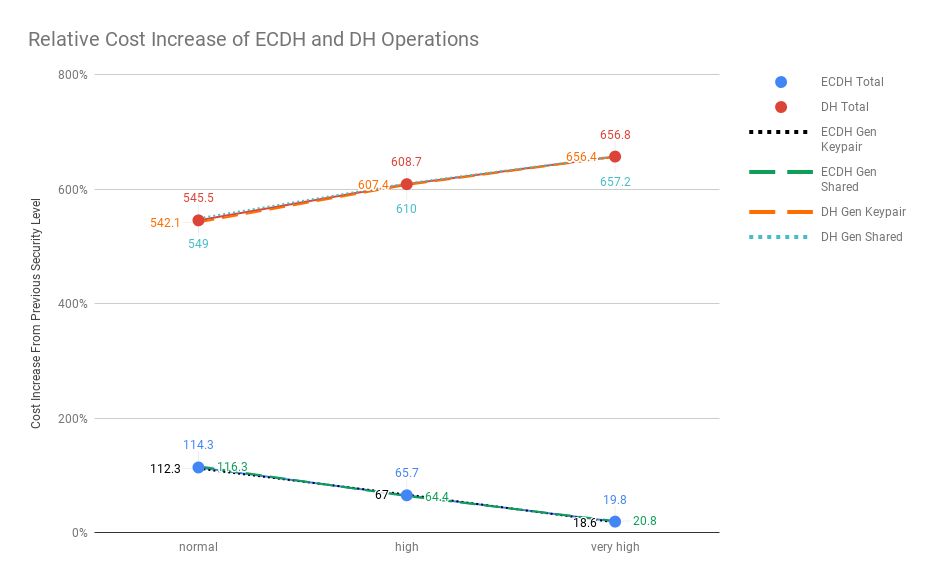
\includegraphics[width=1.0\textwidth]{img/ecdh_dh_relative_cost_increase.png}
    \centering \caption{\label{fig:ecdh-dh-relative-cost-increase} Relative increase of ECDH and DH operation costs}
  \end{figure}

\subsubsection{DH Cost Analysis}

Similarly to \gls{ecdh}, in \gls{dh} two basic operations are performed by each peer: first, a public/private \gls{dh} keypair is generated, followed
by generation of the shared secret, which in \gls{tls}, is used as the premaster secret. Computing the private key is cheap, since it is just a randomly
generated number. The costly part is the computation of the public key and the shared secret, since both of the operations involve modular exponentiations.

We will once again refer to table \ref{table:ecdh-dh-costs-all-sls} for the cost analysis, but this time focusing on \gls{dh}. Figure
\ref{fig:dh-costs-all-sls} shows the costs of \gls{dh}'s operations for all security levels graphically, in logarithmic scale. Just like in \gls{ecdh}, the total cost
is almost evenly divided between the keypair and shared secret generation. This is a consequence of the fact that generating the public/private keys
and the shared secret involves the same type of mathematical operations, thus their costs are similar. An analysis of the figure
also shows that an exponential trendline is the one that best fits the cost increase for all operations.

  \begin{figure}
    \centering
    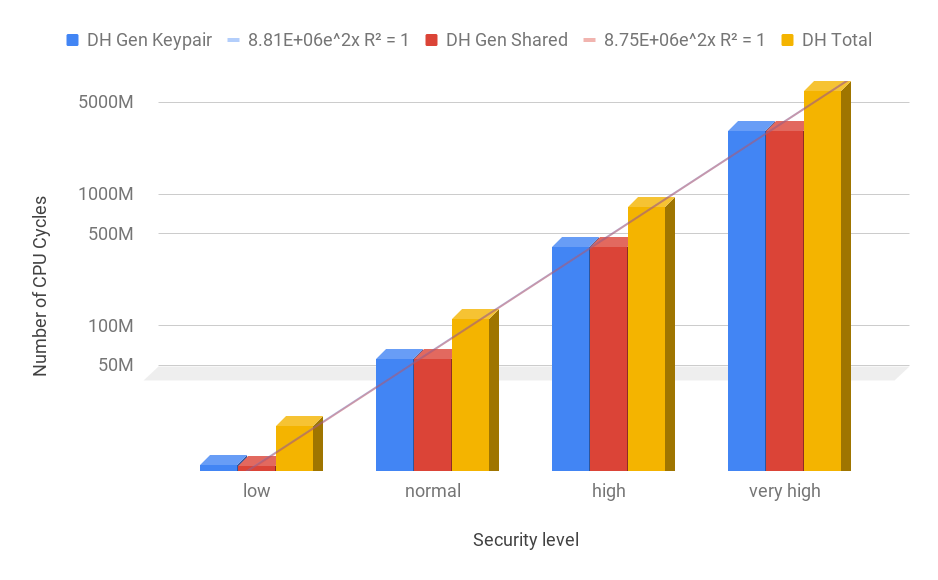
\includegraphics[width=1.0\textwidth]{img/dh_costs_all_sls.png}
    \centering \caption{\label{fig:dh-costs-all-sls} DH operations costs for all security levels (logarithmic scale)}
  \end{figure}

Figure \ref{fig:ecdh-dh-relative-cost-increase} shows the relative cost increase of \gls{dh} operations from the previous security level.
The cost increase of generating the keypair, the shared secret, and consequently of their sum, is very similar, thus the $3$ lines overlap.
As expected, the total relative cost increase represents the average of the values of keypair and shared secret generation relative increase.
An analyzis of figure \ref{fig:ecdh-dh-relative-cost-increase} shows as the security level increases, the relative 
\gls{dh} cost increase becomes larger. In fact, this cost increase is exponential. Although not presented here, this holds true for 
security levels higher than \textbf{very high}. The effect of this exponential increase can be seen in table 
\ref{table:dh-absolute-cost-increase}, which shows the absolute cost increase from the previous security level.

Similarly to \gls{rsa}, \gls{dh} has an exponential cost increase. This similarity is a consequence of both algorithms having the same mathematical
operation at their core: modular exponentiation.

\subsubsection{ECDH vs DH}

Having analyzed the costs of \gls{ecdh} and \gls{dh}, we will now compare them and draw some conclusions. Unlike in our comparison of
\gls{rsa} and \gls{ecdsa} in Section \ref{sec:rsa-vs-ecdsa}, the answer to which one of the algorithms is less costly, is straightforward.
In \gls{rsa} and \gls{ecdsa} the cost the signature creation and verification operations is different, so the choice of the least costly
option depended not only on the security level, but also on whether we were optimizing for the signature creation or verification. In \gls{ecdh} and \gls{dh},
the total cost is almost evenly divided between the keypair and the shared secret generation. Thus, we can make our decision simply
by analyzing table \ref{table:ecdh-dh-costs-total-all-sls} and choosing which algorithm has the smallest value for each security level.
However, in order to simplify the analysis, we have plotted the table \ref{table:ecdh-dh-costs-all-sls} in figure \ref{fig:ecdh-dh-costs-all}, which
presents the data in logarithmic scale.

By looking at figure \ref{fig:ecdh-dh-costs-all} it is easy to see which algorithm has the smallest costs. If the \textbf{low} security level is being used,
\gls{dh} is the least costly choice, if the \textbf{normal} or any security level above is being used, \gls{ecdh} is. Moreover, we can clearly see that
for each algorithm, the costs of their operations is very similar, since we have overlapping lines. The logarithmic and exponential properties of
\gls{ecdh} and \gls{dh}, respectively, are also visible by shape of the lines. Since we are using logarithmic scale for the $y$ axis, the
exponential cost growth of \gls{dh} manifests in the shape of a $y=mx+b$ line.

\begin{figure}
  \centering
  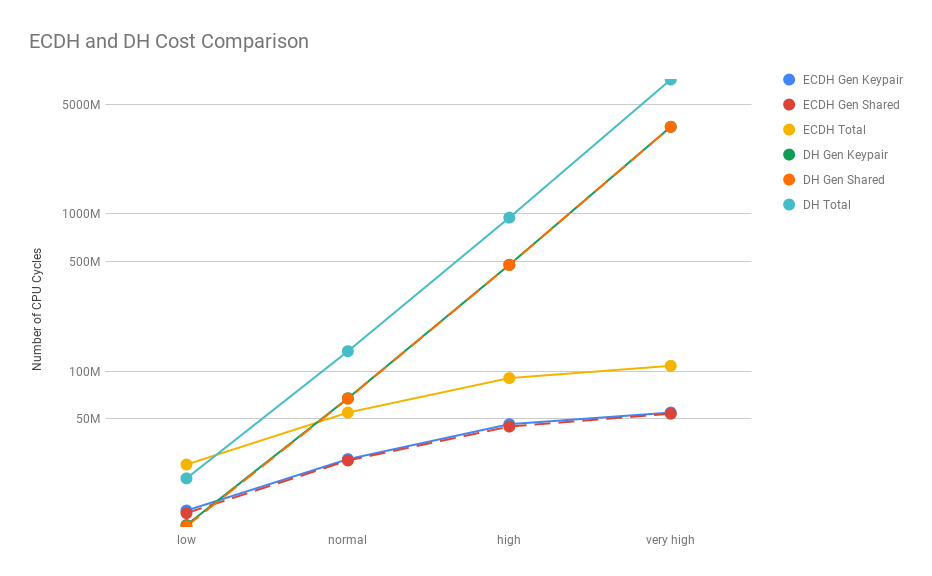
\includegraphics[width=1.0\textwidth]{img/ecdh_dh_costs_all.png}
  \centering \caption{\label{fig:ecdh-dh-costs-all} ECDH and DH cost comparison (logarithmic scale)}
\end{figure}

Although not presented here, the logarithmic and exponential growth trends for \gls{ecdh} and \gls{dh}, respectively, hold true even for
security levels higher than \textbf{very high}. For security levels above \textbf{low}, there are no cost or security
advantages of choosing \gls{dh} over \gls{ecdh}, for either peer. For this reason, for security level above \textbf{low} it makes sense to abandon the
use of \gls{dh}, in favor of \gls{ecdh} completely. As a benefit of removing the \gls{dh} code implementation, the storage footprint will be smaller.

% NOTE: regarding the dhm code size look at mbedtls-2.7.0/library/CMakeFiles/mbedcrypto.dir/dhm.c.o

\subsubsection{The Cost Of PFS In TLS} \label{sec:pfs-cost-in-tls}

Having analyzed the costs of the algorithms that can be used for \gls{pfs}, in this section we will describe the cost of this security service
for each one of the ciphersuites for the client and the server. In order to avoid confusion in the text that follows, it is important to
distinguish the \textit{ECDH} ciphersuite from the \gls{ecdh} algorithm.

In \gls{tls} there are \textit{ECDH} and \textit{ECDHE} ciphersuites. Both use the \gls{ecdh} algorithm, but only \textit{ECDHE} ciphersuites
offer \gls{pfs}. The \textit{E} in \textit{ECDHE} stands for \textit{ephemeral}. While in \textit{ECHDE} ciphersuites, both the client and the server
generate ephemeral \gls{ecdh} parameters, in \textit{ECDH} ciphersuites at least one of the peer's parameters are \textbf{fixed}
within its certificate. In our scenario, only the server authenticates to the client, thus in \textit{ECDH} ciphersuites the server's
\gls{ecdh} parameters will be fixed within its certificate, while the client will have to generate new ones for each connection.
More specifically, in \textit{ECHDE} ciphersuites, with each  new Handshake, both the client and the server generate a new (\textit{i.e.} ephemeral)
public/private \gls{ecc} key pair that will be used with the \gls{ecdh} algorithm. On the other hand, in \textit{ECDH} ciphersuites, only the client
will generate a new public/private \gls{ecc} key pair, since the server's public key is fixed within its certificate. Thus in \textit{ECDH}
ciphersuites, if the server's long-term shared secret, \textit{i.e.} its private \gls{ecc} key, is compromised the previous communication's secrets
can be computed (if the client's public \gls{ecdh} parameters that are sent in the clear are recorded), thus also compromising the confidentiality of
the past communications. The distinction between the \textit{DH} ciphersuite from \gls{dh} algorithm is equivalent. Although \textit{DH} (\textit{i.e}
non-ephemeral \gls{dh}) ciphersuites exist in \gls{tls}, they are not implemented in \textit{mbedTLS 2.7.0}.

Even though the \textit{ECDH} key exchange does not offer \gls{pfs}, it is still closely related to the \textit{ECDHE}, since both use
the \gls{ecdh} algorithm. The additional costs for \textit{ECDH} ciphersuites are significant, and in our evaluated scenario where only the server
authenticates to the client, there is no distinction in costs between \textit{ECDHE} and \textit{ECDH} ciphersuites for the client. Instead of
presenting multiple tables, we decided to show the cost of \gls{pfs} and the \textit{ECDH} key exchange in a single one.

Table \ref{table:pfs-cost-client} shows the cots of \gls{pfs} and the \gls{ecdh} key exchange for the client and table \ref{table:pfs-cost-server}
for the server. As a reminder, only \textit{ECDHE} and \textit{DHE} ciphersuites offer \gls{pfs}. \textit{ECDH-RSA} and \textit{ECDH-ECDSA}
ciphersuites (rows highlighted in gray) do not offer \gls{pfs} and the presented costs are the ones of \textit{ECDH} key exchange. Note, that the
highlighted rows are the only ones whose cost differs for
the client and the server. For the server, the cost of \gls{ecdh} key exchange is the cost of generating the shared secret only.

\begin{figure}
  \centering
  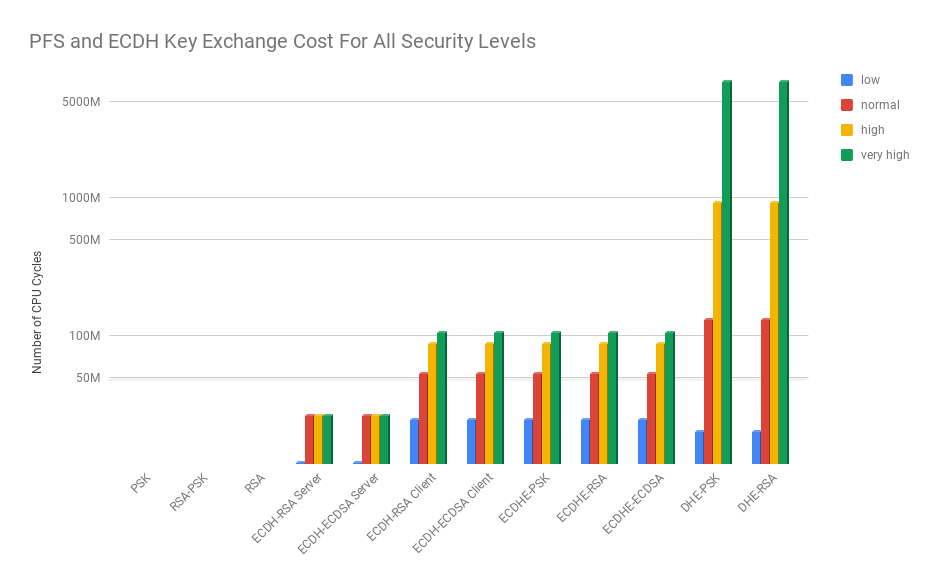
\includegraphics[width=1.0\textwidth]{img/pfs_cost_all_sls.png}
  \centering \caption{\label{fig:pfs-cost-all-sls} \gls{pfs} and \textit{ECDH} key exchange costs (logarithmic scale)}
\end{figure}

Figure \ref{fig:pfs-cost-all-sls} shows the costs of tables \ref{table:pfs-cost-client} and \ref{table:pfs-cost-server} graphically, in logarithmic scale.
 Since the costs
of \textit{ECDH} ciphersuites are the only ones that differ between the client and the server, we decided to present both of the tables in a
single graph. Notice how the costs of \textit{ECDH-RSA} and \textit{ECDH-ECDSA} are distinguished explicitly for the client and the server.
In the figure, we can group the costs into $4$ groups, presented in increasing cost order:

\begin{enumerate}
  \item non-ECDH(E)/DH(E) ciphersuites, which have the total cost of $0$
  \item \textit{ECDH} server-side ciphersuites
  \item \textit{ECDH} client-side and \textit{ECDHE} ciphersuites
  \item \textit{DHE} ciphersuite
\end{enumerate}

In the evaluated scenario, only the server authenticates to the client. If mutual authentication was used (\textit{i.e.} with both, the client
and server authenticating one to another), the costs of \textit{ECDH} ciphersuites would become the same for the client and the server, with the client
having its cost reduced. In the mutual authentication scenario, the client, just like the server, would only have to generate the shared secret, since
its public key would be fixed in its certificate. Thus, the client's \gls{pfs} and \textit{ECDH} costs would be identical to the ones of the server,
presented in table \ref{table:pfs-cost-server}. Figure \ref{fig:pfs-cost-all-sls} would still look the same, except that the client's \textit{ECDH}
ciphersuite costs would become the same as the server's. Thus, the costs could still be separated into the $4$ groups mentioned above,
but now there would be no \textit{ECDH} client/server side separation:

\begin{enumerate}
  \item non-ECDH(E)/DH(E) ciphersuites, which have the total cost of $0$
  \item \textit{ECDH} ciphersuites
  \item \textit{ECDHE} ciphersuites
  \item \textit{DHE} ciphersuite
\end{enumerate}

\subsection{TLS Handshake Cost Analysis} \label{sec:tls-hs-cost}

Having analyzed the costs of the authentication and \gls{pfs} security services in \gls{tls}, we will now put everything together and
analyze the total cost of the handshake. We have already seen the Handshake cost for the \textbf{normal} security level in
Section \ref{sec:ss-overview}. In this section, we will present a more detailed analysis of this and the remaining security levels.

Tables \ref{table:client-hs-cost-all-sls} and \ref{table:server-hs-cost-all-sls} show the average handshake cost for each one of the
key exchange methods, for the client and server, respectively. The number in parenthesis in each table entry is the standard deviation.
The evaluated scenario is the most common one: only the server authenticates to the client.

In \textit{mbedTLS 2.7.0} there is a total of $161$ ciphersuites. Table \ref{table:mbedtls-num-ciphers} shows the number of
ciphersuites per each key exchange method available in \textit{mbedTLS 2.7.0}. For each key exchange method, the average was obtained
from a run with each one of the ciphersuites that use that key exchange.

\begin{table}[]
\begin{tabular}{ll}
\hline
\multicolumn{1}{|l|}{\textbf{Key Exchange}}                     & \multicolumn{1}{l|}{\textbf{Number of Ciphersuites}} \\ \hline
\multicolumn{1}{|l|}{PSK}         & \multicolumn{1}{l|}{19}                        \\ \hline
\multicolumn{1}{|l|}{RSA-PSK}     & \multicolumn{1}{l|}{15}                        \\ \hline
\multicolumn{1}{|l|}{RSA}         & \multicolumn{1}{l|}{23}                        \\ \hline
\multicolumn{1}{|l|}{ECDH-RSA}    & \multicolumn{1}{l|}{13}                        \\ \hline
\multicolumn{1}{|l|}{ECDH-ECDSA}  & \multicolumn{1}{l|}{13}                        \\ \hline
\multicolumn{1}{|l|}{ECDHE-PSK}   & \multicolumn{1}{l|}{11}                        \\ \hline
\multicolumn{1}{|l|}{ECDHE-RSA}   & \multicolumn{1}{l|}{13}                        \\ \hline
\multicolumn{1}{|l|}{ECDHE-ECDSA} & \multicolumn{1}{l|}{17}                        \\ \hline
\multicolumn{1}{|l|}{DHE-PSK}     & \multicolumn{1}{l|}{19}                        \\ \hline
\multicolumn{1}{|l|}{DHE-RSA}     & \multicolumn{1}{l|}{18}                        \\ \hline
Total                                      & 161
\end{tabular}
\centering
\centering \caption{\label{table:mbedtls-num-ciphers} Number of ciphersuites per key exchange method in \textit{mbedTLS 2.7.0}}
\end{table}

Figures \ref{fig:client-hs-cost-all-sls} and \ref{fig:server-hs-cost-all-sls} are a graphical representation of tables \ref{table:client-hs-cost-all-sls}
and \ref{table:server-hs-cost-all-sls}, respectively. The $x$ axis specifies the security level. The $y$ axis presents the number
of CPU cycles used when performing the handshake with the specified key exchange method and security level.
The values are presented in logarithmic scale.  What can be clearly seen in those
graphs, is that even though there are $10$ unique key exchange methods, the costs of some of them overlap, because they are similar.
If two or more key exchange methods have similar costs, we say that they belong to the same \textit{cost group}. A \textit{cost group}
can also contain a single key exchange method, if its costs are significantly different from all others. In figures
\ref{fig:client-hs-cost-all-sls} and \ref{fig:server-hs-cost-all-sls} two or more key exchange methods belong to the same
cost group if their lines overlap throughout all security levels. By analyzing figure \ref{fig:client-hs-cost-all-sls} we can
find $6$ cost groups at the client-side:

\begin{enumerate}
  \item \textit{PSK}
  \item \textit{RSA}, \textit{RSA-PSK}
  \item \textit{ECDHE-PSK}, \textit{ECDHE-RSA}, \textit{ECDH-RSA}
  \item \textit{ECDH-ECDSA}
  \item \textit{ECHDE-ECDSA}
  \item \textit{DHE-PSK}, \textit{DHE-RSA}
\end{enumerate}

Similarly, by analyzing figure \ref{fig:server-hs-cost-all-sls}, we can find $8$ cost groups for the server side:

\begin{enumerate}
  \item \textit{PSK}
  \item \textit{ECDH-RSA}, \textit{ECDH-ECDSA}
  \item \textit{ECHDE-PSK}, \textit{ECDHE-ECDSA}
  \item \textit{RSA}, \textit{RSA-PSK}
  \item \textit{ECDHE-RSA}
  \item \textit{DHE-PSK}
  \item \textit{DHE-RSA}
\end{enumerate}

The groups are presented in ascending cost order. For both, the client and the server, the \textit{PSK} key exchange is, by far,
the cheapest option. The most expensive key exchange method depends on the peer and the security level. If we had to choose one
option for the title of the most expensive one, \textit{DHE-RSA} would be the answer, since this is true starting from
\textbf{normal} security level for the client and \textbf{low} security level for the server. \textit{DHE-PSK} costs come very close, 
especially for the client. Once again we see the advantage of \gls{ecc}, with the cost increase of
key exchanges that use \textit{ECDH(E)} and/or \textit{ECDSA} being much lower than of the ones that use \textit{DHE} and \textit{RSA}
instead. This is a manifestation of logarithmic (for \gls{ecc}) vs exponential (for non-\gls{ecc}) cost increase.

\begin{figure}
  \centering
  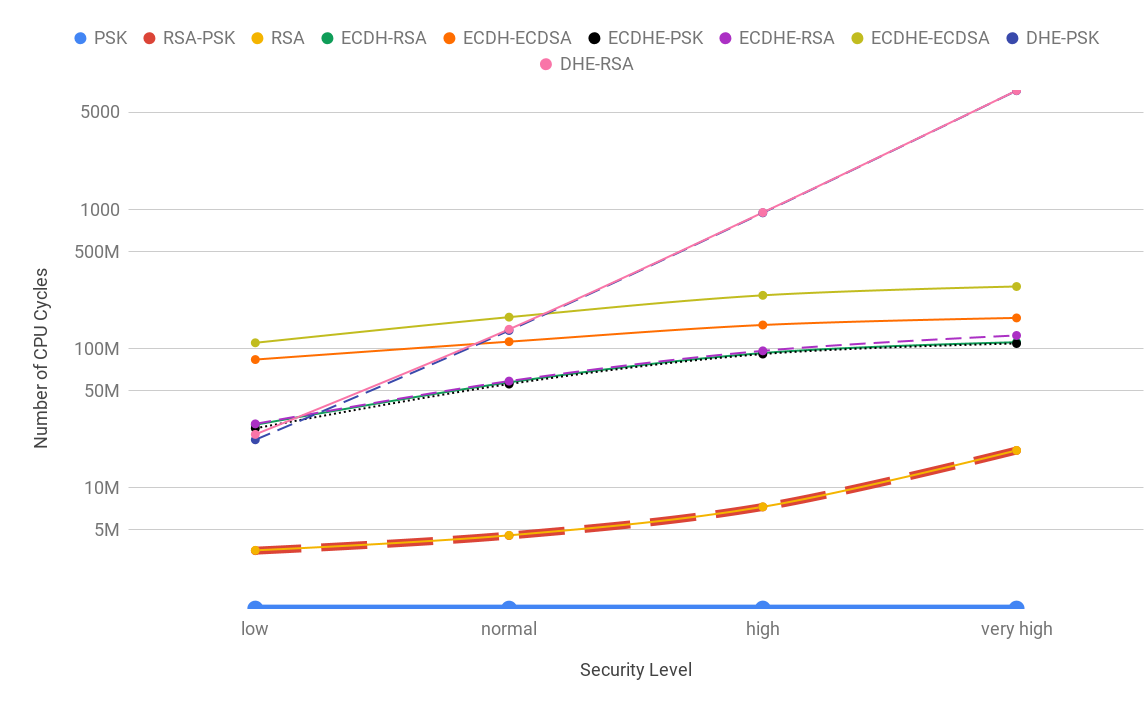
\includegraphics[width=1.0\textwidth]{img/client_hs_costs_all_sls.png}
  \centering \caption{\label{fig:client-hs-cost-all-sls} Client handshake costs for all security levels}
\end{figure}

\begin{figure}
  \centering
  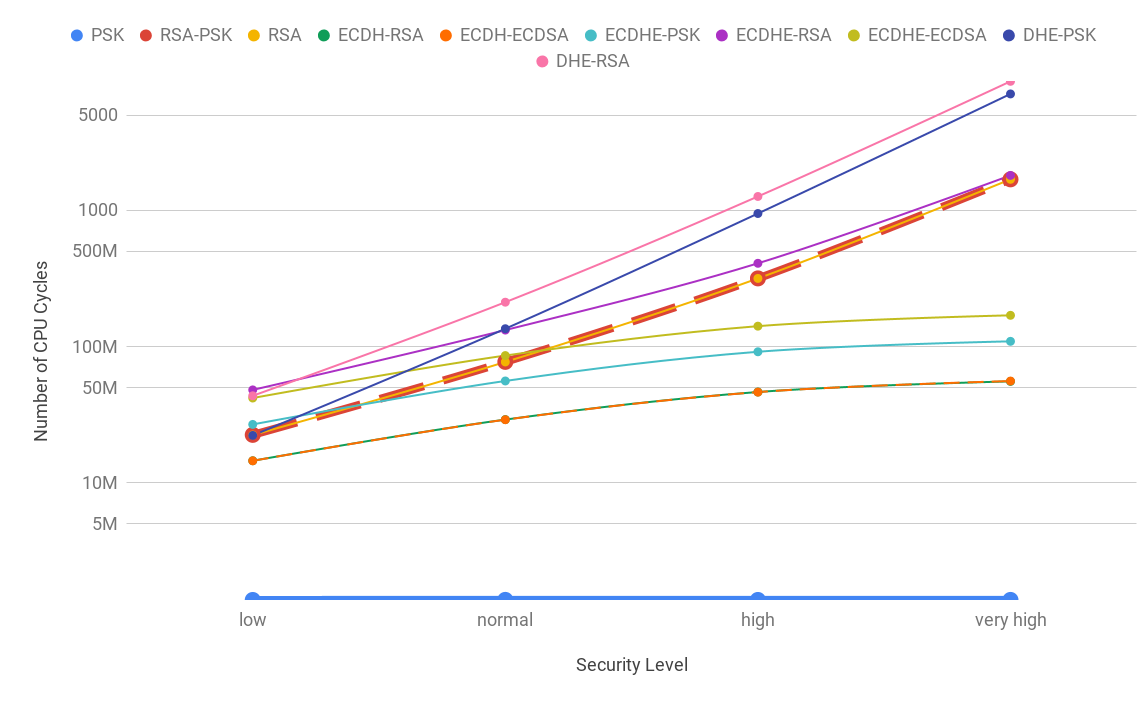
\includegraphics[width=1.0\textwidth]{img/server_hs_costs_all_sls.png}
  \centering \caption{\label{fig:server-hs-cost-all-sls} Server handshake costs for all security levels}
\end{figure}

\begin{table}[]
\begin{tabular}{|l|l|l|}
\hline
\textbf{Key Exchange}                     & \textbf{Asymmetric Auth} & \textbf{PFS} \\ \hline
PSK         & No                       & No           \\ \hline
RSA-PSK     & Yes                      & No           \\ \hline
RSA         & Yes                      & No           \\ \hline
ECDH-RSA    & Yes                      & No           \\ \hline
ECDH-ECDSA  & Yes                      & No           \\ \hline
ECDHE-PSK   & No                       & Yes          \\ \hline
ECDHE-RSA   & Yes                      & Yes          \\ \hline
ECDHE-ECDSA & Yes                      & Yes          \\ \hline
DHE-PSK     & No                       & Yes          \\ \hline
DHE-RSA     & Yes                      & Yes          \\ \hline
\end{tabular}
\centering \caption{\label{table:key-exch-sec-ser} Security services offered by each key exchange}
\end{table}


Due to the constrained nature of \gls{iot} devices, it is important to choose the least costly option for the desired secure
connection properties.
The cost differences between key exchange methods exist for two reasons. First, different key exchange methods offer different
security services. Table \ref{table:key-exch-sec-ser} shows the security services offered by each key exchange method. Second, as
discussed and analyzed throughout Section \ref{sec:auth-cost-in-tls}, different algorithms can be used to offer the same
security service, thus leading to different costs. In order to make a choice of the cheapest key
exchange method, we need to answer $4$ questions:

\begin{enumerate}
  \item what is the desired security level?
  \item do we want to optimize for the client, the server or both?
  \item is asymmetric authentication necessary?
  \item is \gls{pfs} necessary?
\end{enumerate}

Figures \ref{fig:dt-low-sl}, \ref{fig:dt-normal-sl}, \ref{fig:dt-high-sl}, \ref{fig:dt-veryhigh-sl} are decision trees that
help in selecting the cheapest key exchange method for the \textbf{low}, \textbf{normal}, \textbf{high} and \textbf{very high}
security levels, respectively, according to the security requirements. Each on the decision trees answers the $4$ questions
mentioned above. The key exchange methods are presented in order of the cheapest to the most expensive one. If two exchange methods
belong to one of the cost groups presented above, they are are presented as such in the figures too. The cost differences between
the ciphersuites within the same cost group are very small and can be ignored. If the choice is to optimize for the client/server,
ciphersuites are ordered to minimize client/server costs. If the choice is choice is to optimize for both, the
ciphersuite are ordered to minimize the total costs, \textit{i.e.} the sum of the costs for the client and the server.

As an example of how to use the decision trees in order to select the cheapest key exchange method, let us consider the scenario
where the desired security level is \textbf{normal}, asymmetric authentication is required, \gls{pfs} is not and we would like to
minimize the cost for the client. Since the chosen security level is normal, figure \ref{fig:dt-normal-sl} will be used.
We begin at the \textit{Optimize For} node and go left, to follow the \textit{client} path, since that's the peer that we
want to optimize for. Since asymmetric authentication is required, from the \textit{Asymm Auth?} node we follow the \textit{yes}
path. This takes us to the \textit{PFS?} node, where we go right to follow the \textit{no} path, since \gls{pfs} is not required.
We finally arrive at a terminal node which lists the suitable key exchange methods, starting with the cheapest one.
In our case, the least costly key exchange method is either \textit{RSA} or \textit{RSA-PSK}. Both of them belong to the same
cost group for having very similar costs, thus both are presented in the same numeric position. The second least costly option
is \textit{ECDH-RSA}, and the most costly one is \textit{ECDH-ECDSA}. Table \ref{table:client-hs-cost-all-sls} can be consulted for
precise Handshake costs. After making a decision on which key exchange method(s) is(are) acceptable, either one of ciphersuites that
use them can be chosen.

\begin{figure}
  \centering
  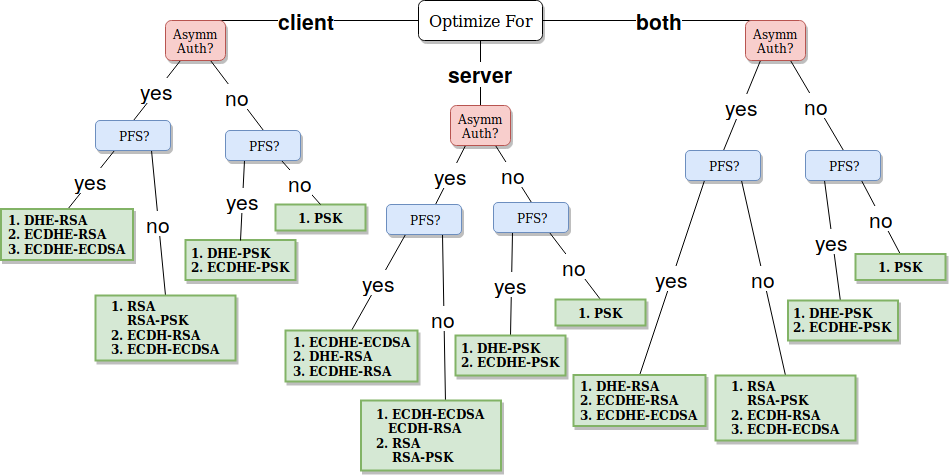
\includegraphics[width=1.0\textwidth]{img/dt_low_sl.png}
  \centering \caption{\label{fig:dt-low-sl} \textbf{low} security level decision tree for the cheapest key exchange}
\end{figure}

\begin{figure}
  \centering
  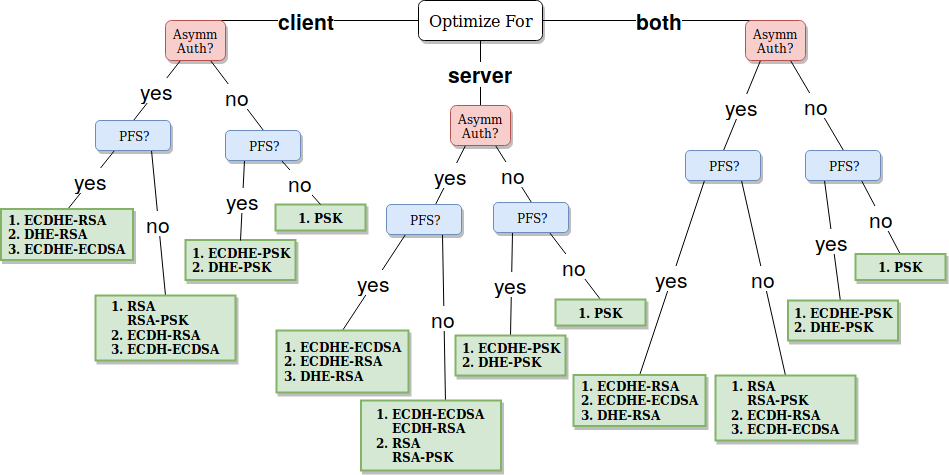
\includegraphics[width=1.0\textwidth]{img/dt_normal_sl.png}
  \centering \caption{\label{fig:dt-normal-sl} \textbf{normal} security level decision tree for the cheapest key exchange}
\end{figure}

\begin{figure}
  \centering
  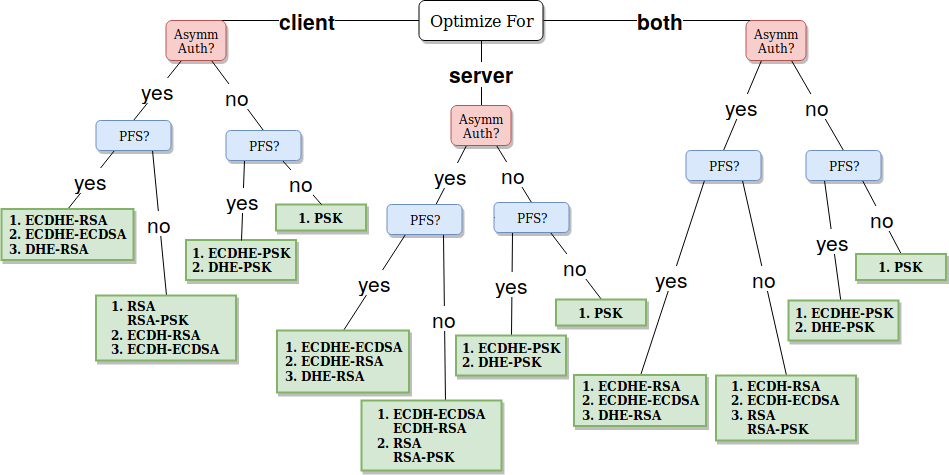
\includegraphics[width=1.0\textwidth]{img/dt_high_sl.png}
  \centering \caption{\label{fig:dt-high-sl} \textbf{high} security level decision tree for the cheapest key exchange}
\end{figure}

\begin{figure}
  \centering
  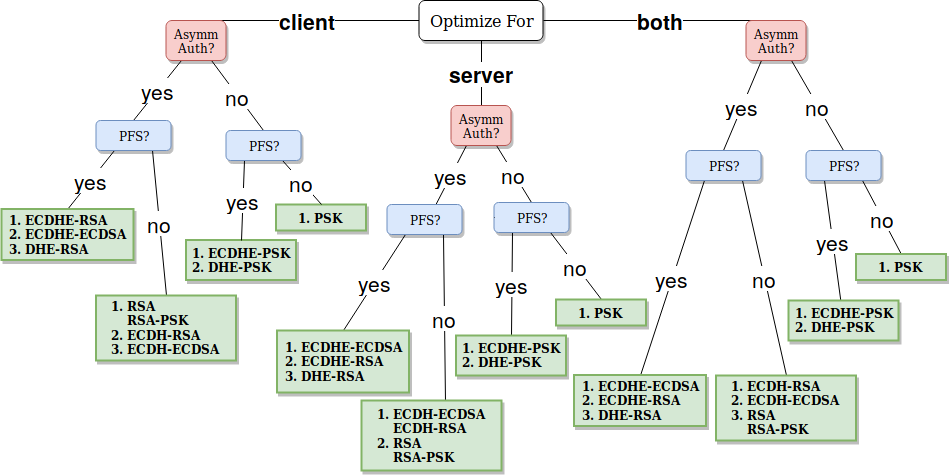
\includegraphics[width=1.0\textwidth]{img/dt_veryhigh_sl.png}
  \centering \caption{\label{fig:dt-veryhigh-sl} \textbf{very high} security level decision tree for the cheapest key exchange}
\end{figure}

In section \ref{sec:auth-cost-in-tls} we analyzed the cost of authentication in \gls{tls} and in section \ref{sec:pfs-cost-in-tls}
the cost of \gls{pfs} in \gls{tls}. Tables \ref{table:tls-auth-cost-client}, \ref{table:pfs-cost-server},
\ref{table:pfs-cost-client} and \ref{table:pfs-cost-server} show the authentication and \gls{pfs} costs for the client and the server,
respectively. However, in order to compute the cost of the Handshake for a given key exchange method and security level, it
is not enough to sum the corresponding values from the authentication and \gls{pfs} cost tables. There is also an overhead of 
establishing the \gls{tls} connection and the parsing/record layer costs. As discussed previously, we can consider the cost of 
the \textit{PSK} handshake as the \gls{tls} overhead.
The parsing and the record layer costs are additional costs that the
peers spend in parsing and reading/writing certain messages not included in the \gls{tls} overhead cost.
Here, reading/writing does not refer to reading/writing to the network, but rather to the record layer. Namely, it is the cost of creating/verifying
the message \gls{mac}. We will refer to those costs as \textit{Additional Costs}.

The majority of the \textit{Additional Costs} come from the \textit{Certificate} message.
This message is omitted entirely in the \textit{PSK} key exchange. In ciphersuites that use asymmetric authentication,
the client has to read the  \textit{Certificate} message from the record layer, parse the \textit{der} encoded certificate into internal fields and
check the validity of its fields, such as the not valid before/after dates. The server has to write the \textit{Certificate} message to the
record layer.

Thus, we can use the following formula to compute the cost of the \gls{tls} Handshake cost for a key exchange method and
security level: $Handshake Cost = TLS Overhead + Auth Cost + PFS Cost + Additional Costs$. The \textit{TLS Overhead} is the cost of the
\textit{PSK} key exchange and can be obtained from table \ref{table:client-hs-cost-all-sls} for the client
and from table \ref{table:server-hs-cost-all-sls} for the server. \textit{Auth Cost} is the cost of authentication and can be obtained
from \ref{table:tls-auth-cost-client} for the client and from table \ref{table:tls-auth-cost-server} for the server. \textit{PFS} cost
is the cost of \gls{pfs} and can be obtained from table \ref{table:pfs-cost-client} for the client and from table \ref{table:pfs-cost-server}
for the server. The majority of \textit{Additional Costs} can be obtained from table \ref{table:cert-parse-cost}, which presents the most relevant
costs when parsing the \textit{Certificate} message.

The certificate is either signed with
\gls{rsa} or \gls{ecdsa}. In \textit{mbedTLS 2.7.0} there are $31$ ciphersuites that use \gls{rsa}-signed certificates and $17$ ciphersuites
that use \gls{ecdsa}-signed certificates. Table \ref{table:cert-parse-cost} contains the cost of parsing the certificate for each algorithm
and security level. This costs do not include checking the certificate's signature, but rather reading the certificate from the record layer,
parsing the \textit{der}-encoded certificate into internal fields, checking the validity of each field and creating a hash of the fields.
The presented values an average of $31$ executions for \gls{rsa} and $17$ for \gls{ecdsa}, each one with a
different ciphersuite. The numbers in parenthesis are standard deviation. An analysis of the table shows that the cost is very similar across all
algorithms and security levels.

\begin{table}[]
\begin{tabular}{|l|l|l|l|l|}
\hline
 \backslashbox{Algorithm}{Security\\Level}              & \textbf{low}   & \textbf{normal} & \textbf{high} & \textbf{very high} \\ \hline
\textbf{RSA}   & 511728 (45373) & 544227 (47594)  & 607542 (51576) & 735237 (59853)      \\ \hline
\textbf{ECDSA} & 548841 (45064) & 662348 (45175) & 666866 (45923)  & 704135 (48247)        \\ \hline
\end{tabular}
\centering \caption{ \label{table:cert-parse-cost} Additional costs of parsing the certificate}

\end{table}

As an example, we will compute the client's Handshake cost for the \textbf{high} security level with \textit{ECHDE-RSA}
key exchange, from the \gls{tls} security service costs that we presented in sections \ref{sec:auth-cost-in-tls} and \ref{sec:pfs-cost-in-tls}.
First, we will need to get the \textit{TLSOverhead} value. We can obtain in from the entry located at the
\textit{ECDHE-RSA} row and \textit{high} column in table \ref{table:client-hs-cost-all-sls}: $1355005$. \textit{AuthCost} can be obtained
from the \textit{ECDHE-RSA} row and \textit{high} column in table \ref{table:tls-auth-cost-client}: $4413164$. Similarly \textit{PFSCost}
can be obtained from table \ref{table:pfs-cost-client}, where the \textit{PSK} row and \textit{high} column intersect: $90231688$.
For the additional certificate parsing costs, we will consult table \ref{table:cert-parse-cost}. Since the certificate is an \gls{rsa} signed one,
we will use the value from \textit{RSA} row and \textit{high} column: $607542$. All that's left now is insert those values in the formula:
$Handshake Cost = TLS Overhead + Auth Cost + PFS Cost + Additional Costs = 1355005 + 4413164 + 90231688 + 607542 = 96607399$.

This value was obtained by decomposing the \gls{tls} Handshake into the security services and adding up their costs. As we can see,
the cost computed using the formula is very close to the actual Handshake cost when evaluated as a whole,
which can be found in in table \ref{table:client-hs-cost-all-sls} (\textit{ECDHE-RSA} row and \textit{high} column): $96730901$.
The difference of $123502$ ($96730901-96607399$) CPU cycles comes from other additional costs, such as reading and writing slightly larger
messages, namely the \textit{ServerKeyExchange} and the \textit{ClientKeyExchange}.

\subsection{Confidentiality and Integrity Cost Analysis} \label{sec:confid-costs}

Having analyzed the cost of authentication and \gls{pfs}, we will now briefly analyze the cost of the confidentiality and integrity services.
In \gls{tls}, it does not make sense to analyze both of the services separately, since they're offered as a whole as a part of the ciphersuite.
For this reason, we will analyze them together.

In \textit{mbedTLS 2.7.0} implements $13$ non-null unique encryption algorithms and $4$ unique hash functions. There are $6$ \textit{AES} 
algorithms, $4$ \textit{CAMELLIA} algorithms,
$1$ \textit{DES} algorithm, $1$ \textit{3DES} algorithm and $1$ \textit{RC4} algorithm. The $4$ available hash functions are \textit{SHA-1}, 
\textit{SHA-256}, \textit{SHA-384} and \textit{MD5}.
For non-\gls{aead} ciphers, the combination of a symmetric encryption algorithm and a hash function is used to provide the security services of confidentiality and 
integrity. For \gls{aead} ciphers the symmetric encryption algorithm provides both, confidentiality and integrity, so there is no need
to use an additional hash function.

\begin{figure}
  \centering
  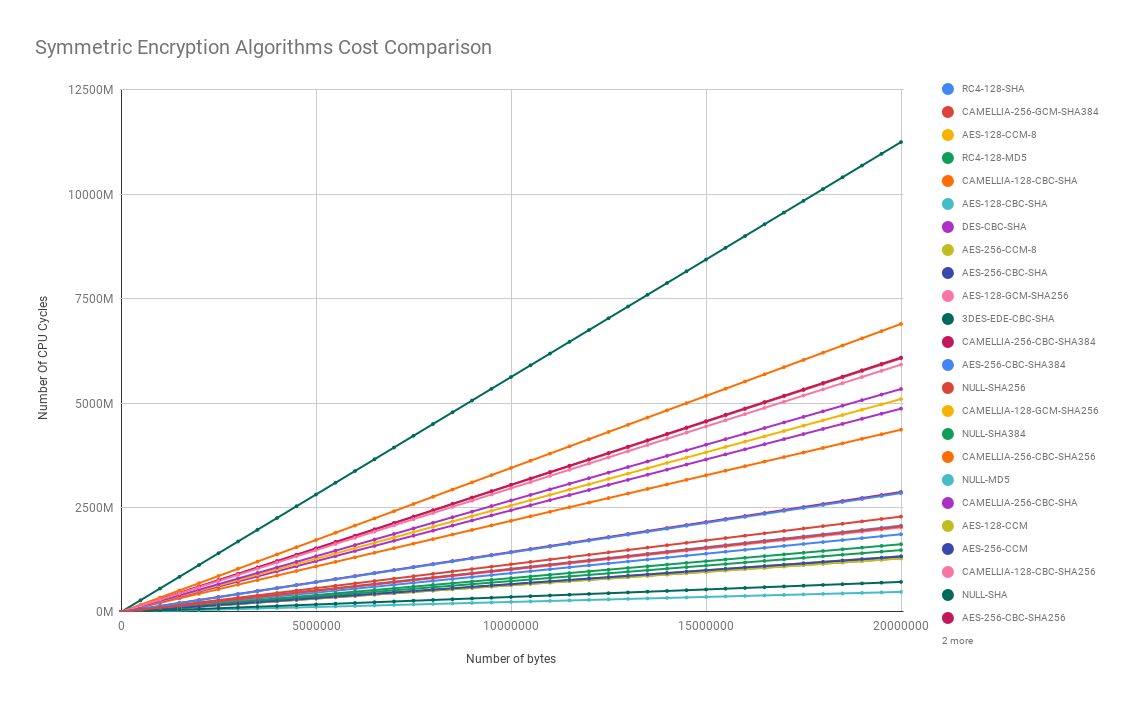
\includegraphics[width=1.0\textwidth]{img/sym_algs_cc.png}
  \centering \caption{\label{fig:symm-encr-all} Confidentiality and integrity cost with different algorithms}
\end{figure}

Figure \ref{fig:symm-encr-all} shows the cost of encryption and \gls{mac} creation using each one of the $26$ symmetric encryption 
algorithm/hash function pairs available in \textit{mbedTLS 2.7.0}. As expected, their cost grows linearly with the amount of encrypted bytes.
An analysis of the graph shows that \textit{3DES} with \textit{SHA} is the most costly combination of an encryption algorithm with a \gls{mac} function, 
while \gls{aead} encryption algorithms 
(\textit{AES} with \textit{GCM} and \textit{CCM} modes) are the least costly block cipher algorithms. 
\textit{CAMELLIA} algorithms are more costly than their \textit{AES} counterparts.  The cost of integrity without encryption can be seen by looking at the null
encryption ciphersuites: \textit{NULL-MD5}, \textit{NULL-SHA}, \textit{NULL-SHA256} and \textit{NULL-SHA384}.
For both, \gls{aead} algorithms and non-\gls{aead} algorithms combined with a hash function, the majority of the cost comes from data encryption.

In Section \ref{sec:tls-hs-cost} we analyzed the cost of the handshake. However, it only makes sense to heavily optimize handshake
if the amount of transmitted data is small. This is, in fact, true for many \gls{iot} devices. But what exactly is a \textit{small} amount of data?

In order to answer those questions we profiled the costs of encrypting data with the \textit{AES-128-GCM} (\textbf{low} and 
\textbf{normal} security levels) and \textit{AES-256-GCM} (\textbf{high} and \textbf{very high} security levels). 
We selected those algorithms because they were among the cheapest ones to provide the required security level and are preferred by
browsers, such as \textit{Google Chrome 67}. The cost of encryption and decryption for those algorithms are similar\cite{ertaul2016performance}.
For each
one of the algorithms, we encrypted data sizes from starting from $1$ byte up to $16250000$ bytes (approximately $15.5$ mega bytes),
with $100$ byte increments in each run. Thus, a total of $162500$ runs was made with each algorithm. It is expected for encryption costs to
grow linearly with the amount of encrypted data, thus we applied linear regression to the collected metrics in order in order to
obtain a formula that approximates the cost of encryption for any amount of data. Our analysis yielded the following formulas for the
cost of encryption with \textit{AES-128-GCM} and \textit{AES-256-GCM}, respectively: $NumCC=104*NumBytes+22680$ and $NumCC=105*NumBytes+22740$ ($R²=1$ for both).
$NumCC$ is the number of CPU Cycles and $NumBytes$ is the number of bytes encrypted. As we cam see. the cost of \textit{AES-256-GCM} is slightly
larger than of \textit{AES-128-GCM}.

The derived formulas can be used to answer the question of when the costs spent on data encryption equate the costs
spent on performing the handshake. For example, let's compute this number for the client, when it performs an
\textit{ECDHE-ECDSA} handshake at the \textit{normal} security level. First, we obtain the number of CPU cycles
used to perform the handshake from table \ref{table:client-hs-cost-all-sls}: $168954007$. After that we simply
replace $NumCC$ with that value in the formula and solve for $NumBytes$: $168954007=104*NumBytes+22680 \Leftrightarrow NumBytes \approx 1624340$.
Thus, the client needs to send $1624340$ bytes ($\approx 1.5$ mega bytes) for the encryption costs to equate the \textit{ECDHE-ECDSA} handshake cots.

Figures \ref{fig:cli-conf-hs-low}, \ref{fig:cli-conf-hs-normal} and \ref{fig:cli-conf-hs-high} help to visualize when
when the encryption/decryption costs equate the handshake costs for the \textbf{low}, \textbf{normal} and \textbf{high}
security levels, respectively. Figures \ref{fig:srv-conf-hs-low}, \ref{fig:srv-conf-hs-normal} and \ref{fig:srv-conf-hs-high}
show the same information for the server. We did not present the graphs for the \textit{very high} security level,
because the overwhelming cost of some key exchange methods made the visual analysis of the graph hard (due to scale).

\begin{figure}
  \centering
  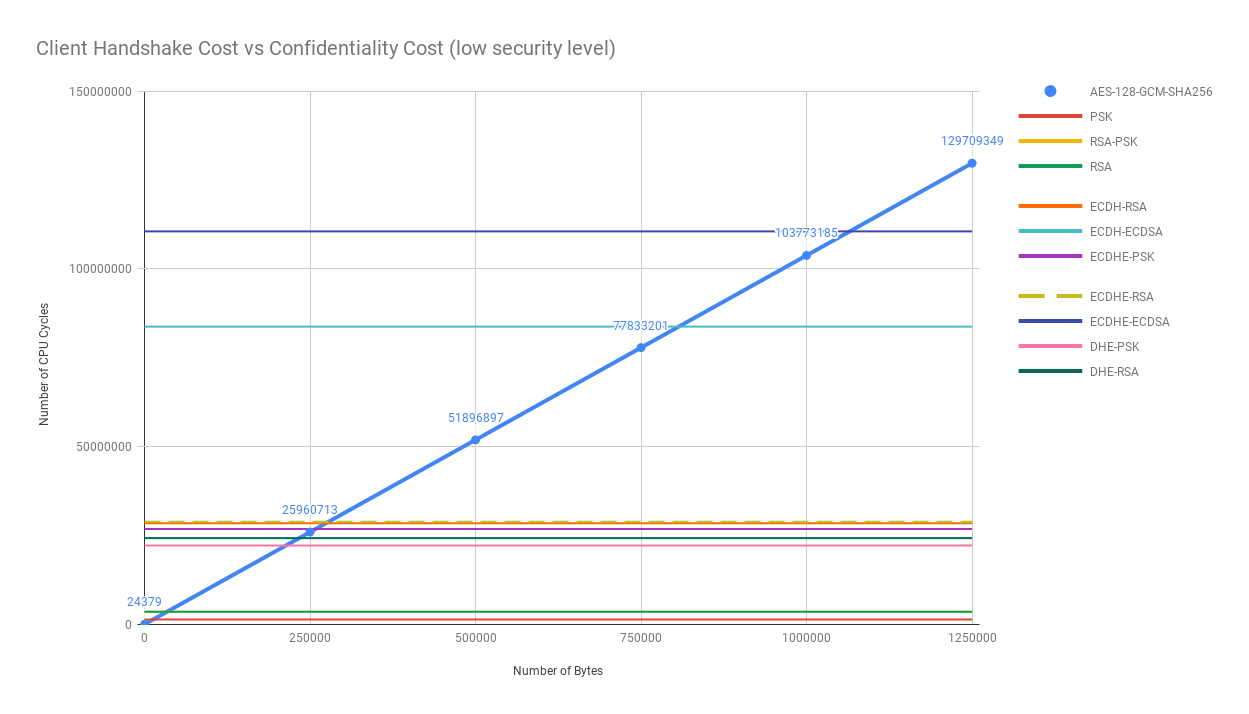
\includegraphics[width=1.0\textwidth]{img/cli_conf_hs_low.png}
  \centering \caption{\label{fig:cli-conf-hs-low} Client handshake vs confidentiality cost for the \textbf{low} security level}
\end{figure}

\begin{figure}
  \centering
  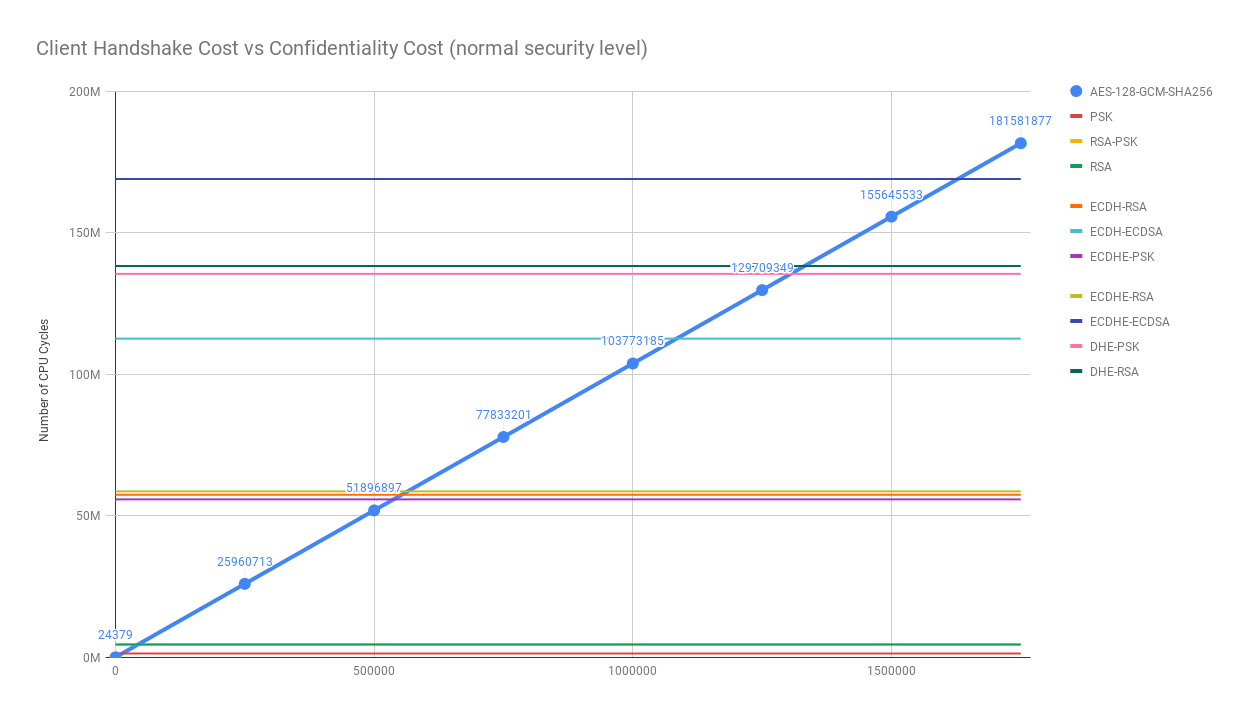
\includegraphics[width=1.0\textwidth]{img/cli_conf_hs_normal.png}
  \centering \caption{\label{fig:cli-conf-hs-normal} Client handshake vs confidentiality cost for the \textbf{normal} security level}
\end{figure}

\begin{figure}
  \centering
  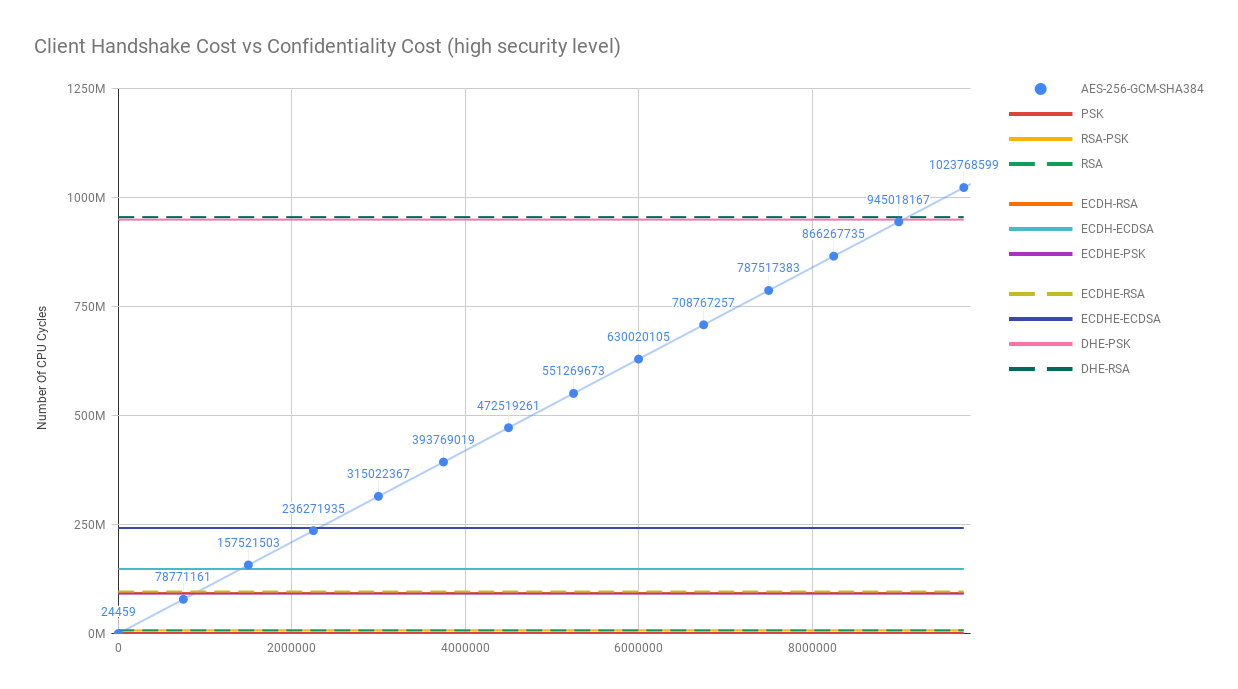
\includegraphics[width=1.0\textwidth]{img/cli_conf_hs_high.png}
  \centering \caption{\label{fig:cli-conf-hs-high} Client handshake vs confidentiality cost for the \textbf{high} security level}
\end{figure}

\begin{figure}
  \centering
  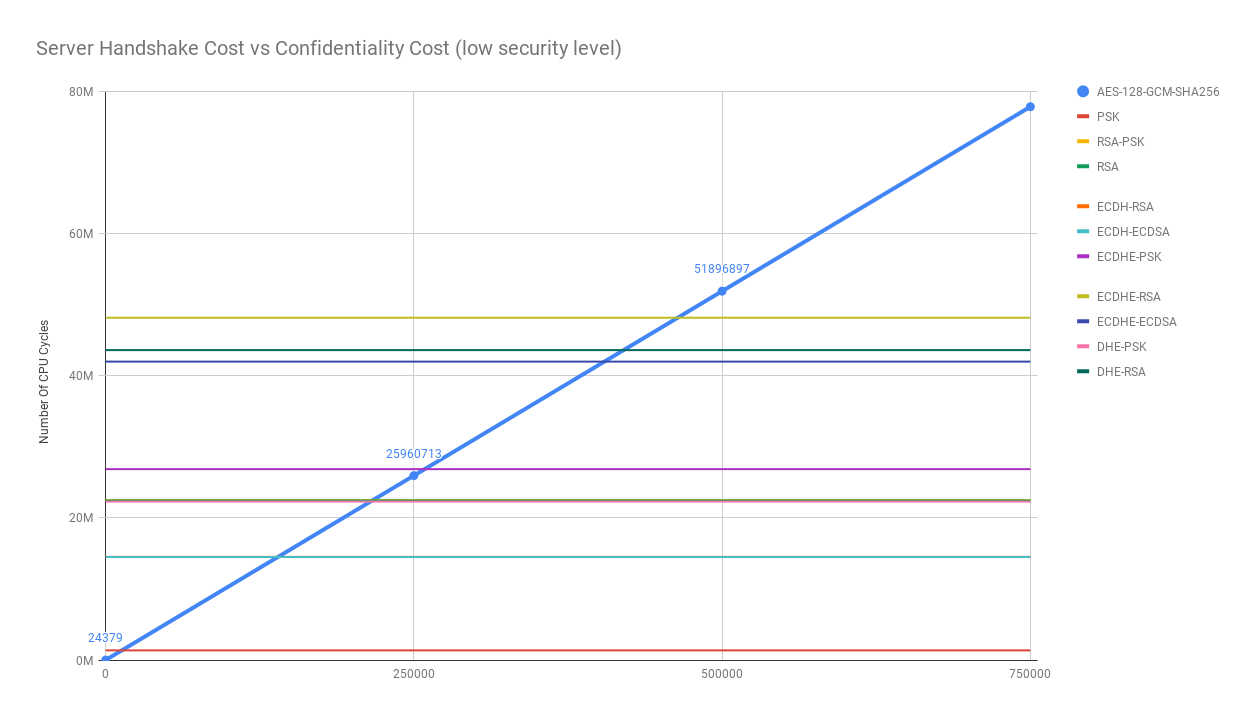
\includegraphics[width=1.0\textwidth]{img/srv_conf_hs_low.png}
  \centering \caption{\label{fig:srv-conf-hs-low} Server handshake vs confidentiality cost for the \textbf{low} security level}
\end{figure}

\begin{figure}
  \centering
  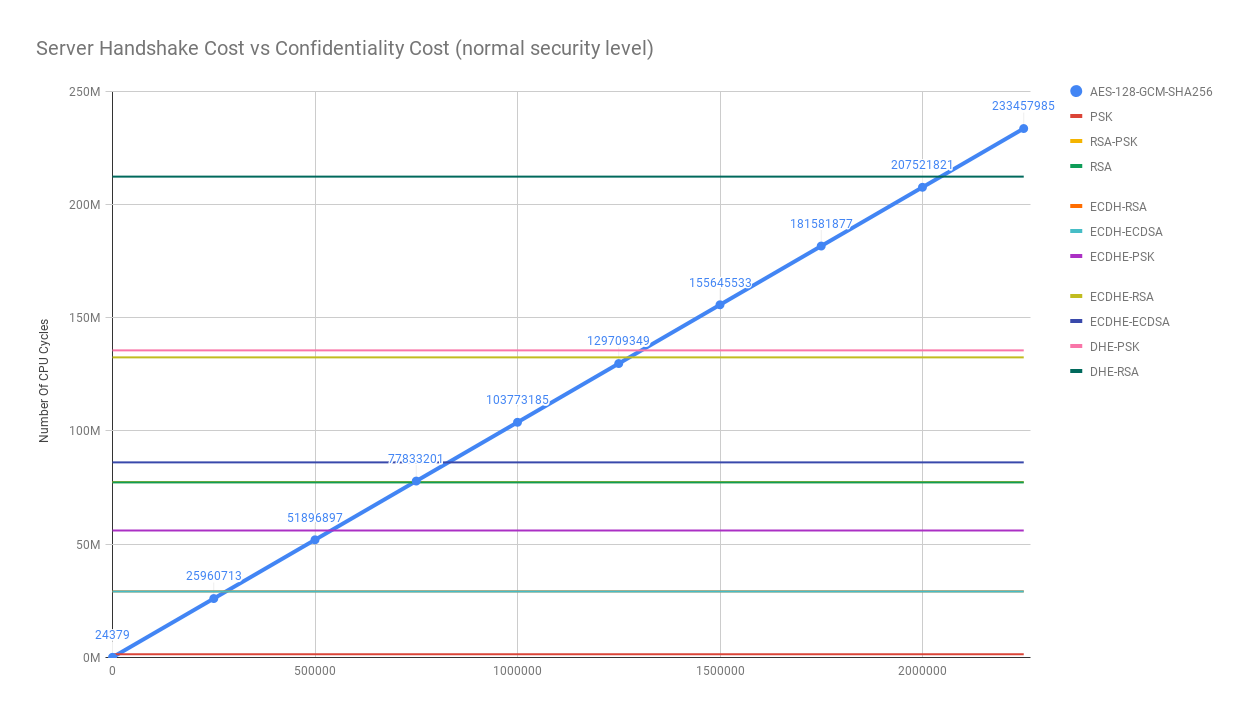
\includegraphics[width=1.0\textwidth]{img/srv_conf_hs_normal.png}
  \centering \caption{\label{fig:srv-conf-hs-normal} Server handshake vs confidentiality cost for the \textbf{normal} security level}
\end{figure}

\begin{figure}
  \centering
  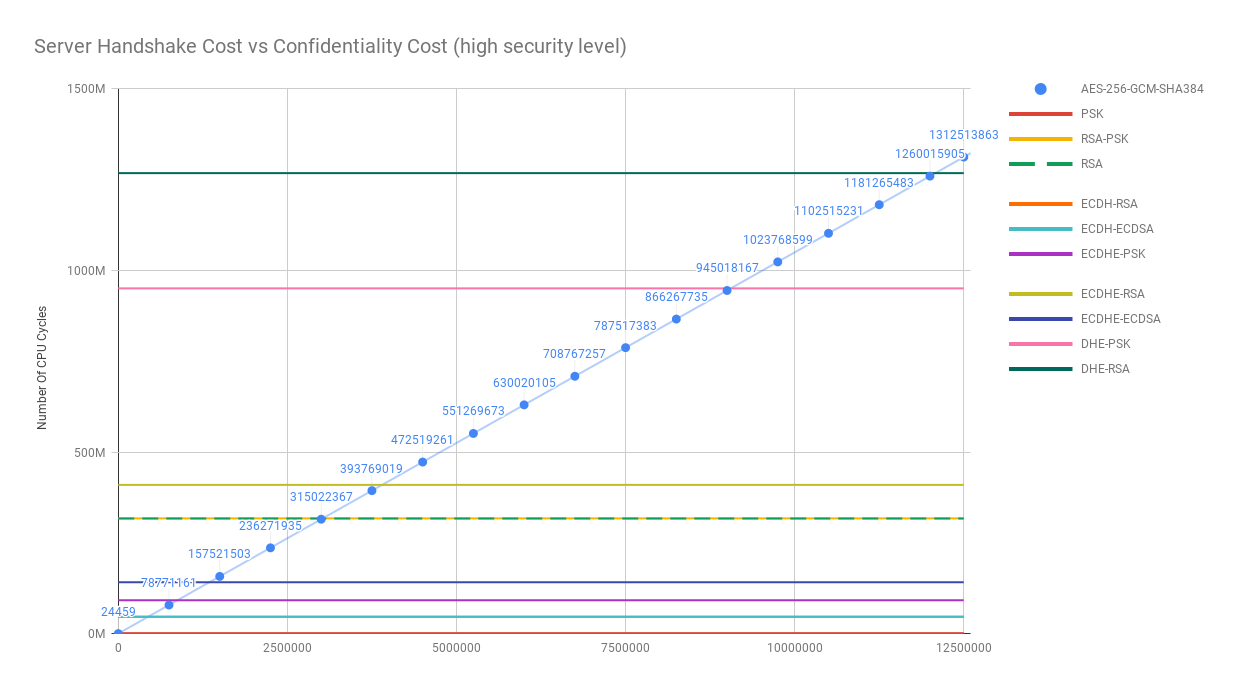
\includegraphics[width=1.0\textwidth]{img/srv_conf_hs_high.png}
  \centering \caption{\label{fig:srv-conf-hs-high} Server handshake vs confidentiality cost for the \textbf{high} security level}
\end{figure}


\subsection{PAPI Time Cost Analysis and Comparison To Estimated CPU Cycles }

We also used \gls{papi} to measure time. In this section, we will compare the estimates of the number of CPU cycles
obtained with \textit{valgrind} with the time values obtained with \gls{papi}. In order to obtain the time metrics with
\gls{papi} we used the same approach and the same number of runs as with \textit{valgrind}. The 

\textit{The iron law of processor performance}\cite{yadin2016computer} states that the time
taken by a program execution is proportional to the number of instuctions (\textit{I}), 
the average number of cycles per instruction (\textit{CPI}) and the amount of time per each processor
cycle (\textit{CT}): $CPU Time = I * CPI * CT$. The number of CPU cycles can be approximated as 
follows: $CPU Cycles = I * CPI$. This means taht the program execution time can be expressed 
as a product of the number of CPU cycles and a constant: $CPU Time = CPU Cycles * CT$.
Thus, we expect the graphs with time in the $y$ axis to look similar, but have smaller
values. The results obtained with \gls{papi} matched our expectations.

\subsubsection{Handhsake Time Cost Analysis} \label{sec:papi-handshake}

\begin{figure}
  \centering
  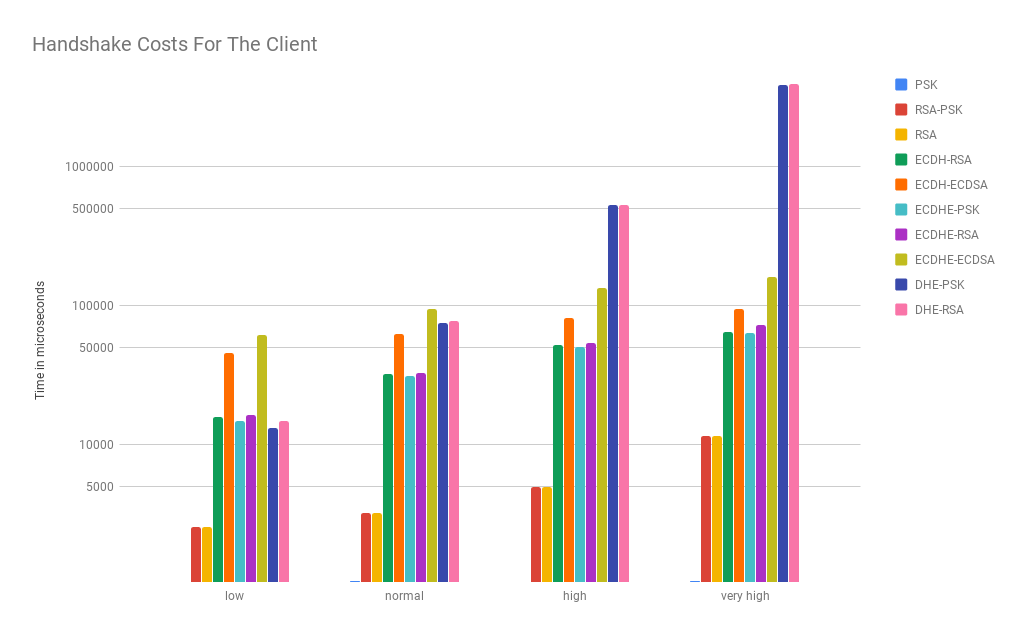
\includegraphics[width=1.0\textwidth]{img/hs_papi_client.png}
  \centering \caption{\label{fig:client-hs-cost-all-sls-papi} Client handshake cost in microseconds for all security levels (logarithmic scale)}
\end{figure}

\begin{figure}
  \centering
  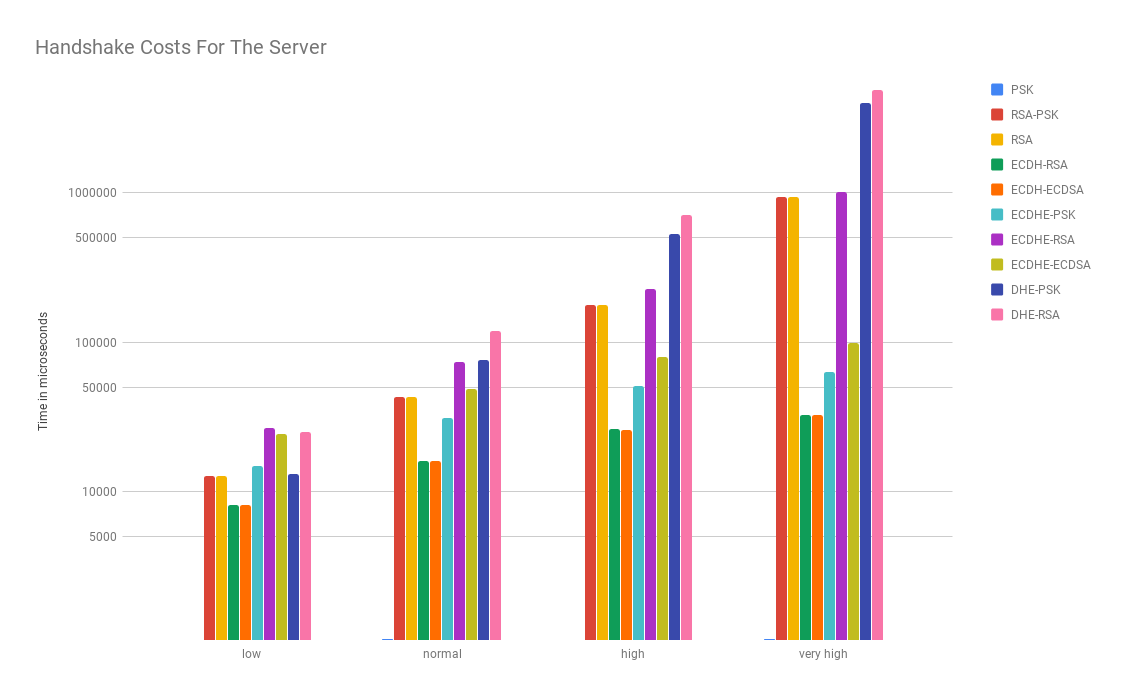
\includegraphics[width=1.0\textwidth]{img/hs_papi_server.png}
  \centering \caption{\label{fig:server-hs-cost-all-sls-papi} Server handshake cost in microseconds for all security levels (logarithmic scale)}
\end{figure}

Figures \ref{fig:client-hs-cost-all-sls-papi} and \ref{fig:server-hs-cost-all-sls-papi} show the time taken to preform the handshake with each one
of the ciphersuites, for each one of the security levels. The $x$ axis specifies the security level. The $y$ axis specifies the time taken in microseconds,
when performing the handshake with the specified key exchange method and security level. The values are presented in logarithmic scale. A comparison of
\ref{fig:client-hs-cost-all-sls-papi} to \ref{fig:client-hs-cost-all-sls} and of \ref{fig:server-hs-cost-all-sls-papi} to \ref{fig:server-hs-cost-all-sls-papi} shows that they look identical,
differing only on the $y$ values. This holds true not only for the overally \textit{handshake} cost, but for all other costs that we analyzed as well. The ratio between
each realted set of operations is also similar.

\subsubsection{PAPI and Valgrind Ratios Comparison} \label{sec:papi-valgrind-ratios}


\begin{figure}
  \centering
  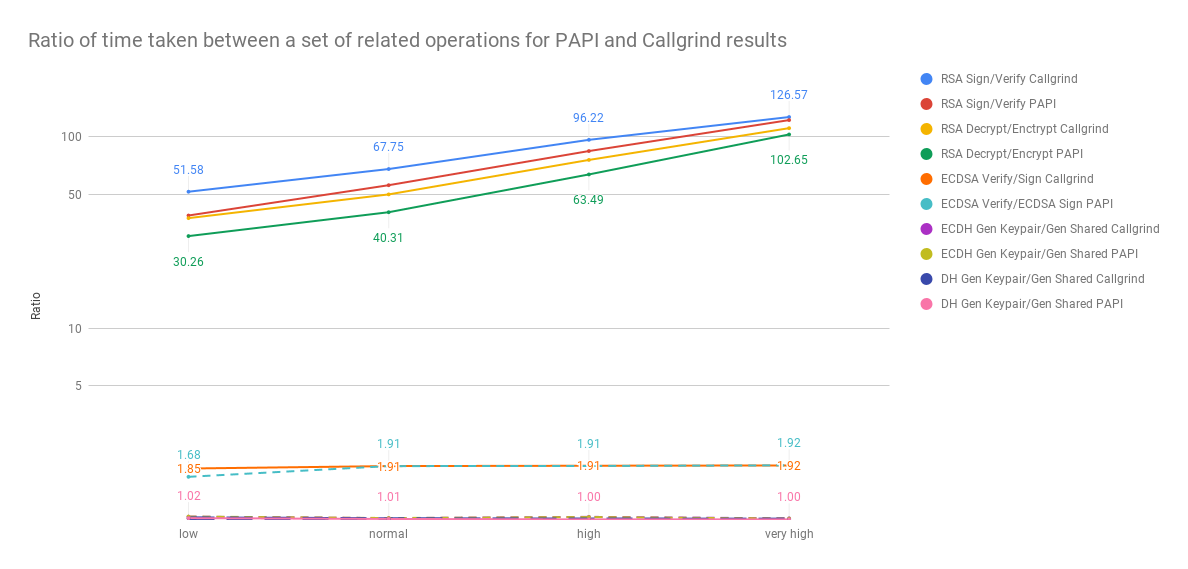
\includegraphics[width=1.0\textwidth]{img/papi-ratio.png}
  \centering \caption{\label{fig:papi-operations-ratio} Ratio of time taken between a set of related operations for \gls{papi} and \textit{callgrind} (logarithmic scale)}
\end{figure}

Figure \ref{fig:papi-operations-ratio} depicts the ratio between \gls{rsa} signature creation and verification, \gls{rsa}
encryption and decryption, \gls{ecdsa} signature verification and creation, \gls{ecdh} keypair and shared secret generation and
\gls{dh} keypair and shared secret generation for both, \textit{valgrind} and \gls{papi}. We purpusefuly devided the more
costly operation by the least costly one, so that all of the ratios are positive. The results are presented in logarithmic scale. An analysis of the figure shows that
both, the \textit{valgrind} and the \gls{papi} ratios are very similar. This is specially true for the \gls{ecdh}, \gls{dh}
and \gls{ecdsa}. For \gls{dh} there is no difference, for \gls{ecdh}, \textit{callgrind}'s ratio is $0.96\%$ larger at the \textit{high} and
\textit{very high} security levels, and for \gls{ecdsa} the ratio differs only for the \textit{low} 
security level, where it's $9.2\%$ larger in \textit{callgrind} than in \textit{papi}. The largest difference in ratio
is observed for opeartions that use \gls{rsa}, but this difference gets smaller as the security level increases. In fact,
this is the general trend for all of the cases. \textit{callgrind}'s \gls{rsa}'s sign/verify ratio is $24.87\%$ larger than \gls{papi}'s
for the \textit{low} security level this differnce is only $3.6\%$. Following the trend, \textit{callgrind}'s \gls{rsa}'s encrypt/decrypt ratio is $19.41\%$ higher
than \textit{papi}'s for the low security level, and $7.3\%$ higher for the \textit{high} security level.

Given that the ratios described above are similar, the algorithm cost comparisons for the various security levels remain valid for \gls{papi}'s time values as well.
Consequently, this is also true for the security services, since they are composed of those algirithms. The graphs for the security services and algorithms look very similar
the \textit{valgrind} ones, for this reason, they have been included in the annex without any further analysis.

\subsection{Discussion} \label{sec:ss-cost-conclusions}

In this section evaluated the cost of security services of authentication, \gls{pfs}, confidentiality and integrity
in \gls{tls}. To do this, we defined $4$ security levels and analyzed the costs for each one. The majority of
analysis was focused on the handshake and the security services that it offers. We did performed the analysis at
two levels: first by using the estimated number of CPU cycles obtained with \textit{valgrind}, and then using the
execution time values obtained with \gls{papi}.

In \gls{tls} there are two ways of doing authentication: \gls{psk} or asymmetric cryptography. We showed that the
cost of \gls{psk} authentication is essentially $0$ and we can consider the cost of performing the 
handshake with a \textit{PSK} ciphersuite can be considered as the \gls{tls} overhead.

In \gls{tls}, authentication with asymmetric cryptography can be done in two ways: either by using \gls{rsa}
of \gls{ecdsa}. We began by analyzing the costs of those two algorithms. We concluded that \gls{rsa} was
faster at public key operations (\textit{i.e.} signature verification) and \gls{ecdsa} was faster at private key
operations (\textit{i.e.} signature creation). An analyzes of the algorithm's costs showed that as the security level
increases, while \gls{rsa}'s cost increase exponentially, \gls{ecdsa}'s increase logarithmically. This is a result of the
\gls{ecc} properties of the algorithm.

After evaluating the costs of individual algorithms that can be used to provide asymmetric authentication in \gls{tls}, we
used those results to compute the authentication cost in \gls{tls}, for each one of its key exchange methods.

After analyzing the cost of authentication, we turned our attention to \gls{pfs}. In \gls{tls} there are two ways
of achieving \gls{pfs}: either by using \gls{ecdh} or \gls{dh}. We decomposed each algorithm into individual steps
and analyzed their cost. As the security level increases, the cost of \gls{dh} grows exponentially, while the cost
of \gls{ecdh} logarithmically. In that sense, \gls{dh} is similar to \gls{rsa} and \gls{ecdh} to \gls{ecdsa}.
This similarity is a consequence of the fact, the underlying mathematical operation is the same for \gls{dh} and
\gls{rsa} (modular exponentiation), and for \gls{ecdh} and \gls{ecdsa} (multiplication of a scalar by a point on 
the elliptic curve). After evaluating the costs of the algorithms that can be used to provide \gls{pfs} in \gls{tls}, we used those results
to arrive at \gls{pfs} cost for each on of the key exchange methods.

Having computed the costs of authentication and \gls{pfs} we were now ready to compute the cost of the \gls{tls} handshake
as a whole. We presented a formula that decomposed the handshake costs its individual parts: $Handshake Cost = TLS Overhead + Auth Cost + PFS Cost + Additional Costs$. 
We compared the costs
obtained from the formula to the actual handshake cost values that we acquired by profiling various client-server
executions and showed that both are similar.

Finally, we analyzed the costs of confidentiality and integrity. First, we compared the costs of all of the
symmetric algorithm/hash function combinations available in \textit{mbedTLS 2.7.0}. As expected,
\gls{aead} algorithms preformed the best among the block ciphers. After that we chose two \gls{aead} ciphers and
analyzed how much data it would be necessary to encrypt with them to equate the handshake costs.

The analysis the \gls{papi} results showed us that the estimates obtained with \textit{valgrind} do reflect the real world values. 
Not only the higher-level results are similar in comparison to one another, but at the lower level, the ratios between the algorithms 
used by the security services also are. As the \textit{The iron law of processor performance} suggested, the time values can be approximated as 
the estimated number of CPU cycles multiplied by a factor smaller than $1$. Thus, the estimates from the previous sections can be used for 
relative comparisons between the costs of security services and security levels in \gls{tls}, thus allowing to achieve the goals of this work. 
The time costs presented in this seciton and in the Annex provide concrete, real-world reference values for the costs of the various parts of 
the \gls{tls} protocol.